%
% IzPack documentation
%
% Copyright (c) 2001, 2002 Julien Ponge
%
% <julien@izforge.com>
% http://www.izforge.com/
%
%begin{latexonly}
\newif\ifpdf
\ifx\pdfoutput\undefined
\pdffalse
\else
\pdfoutput=1
\pdftrue
\fi

% Change this as needed :
%   - a4paper to your paper format
%   - the document class to your need (book, article, ...)
\ifpdf
\documentclass[a4paper, 12pt, pdftex]{report}
\else
%end{latexonly}
\documentclass[a4paper, 12pt, dvips]{report}
%begin{latexonly}
\fi
%end{latexonly}

% The packages we need
\usepackage{verbatim}
\usepackage{moreverb}
\usepackage{url}
\usepackage{tabularx}
\usepackage[final]{graphicx}
\usepackage[hyperindex,breaklinks=true,pdfborder={0 0 0}]{hyperref}
%begin{latexonly}
\ifpdf
\hypersetup{colorlinks=true,linkcolor=blue,urlcolor=blue,citecolor=red}
\fi
%end{latexonly}
\usepackage{html}
\begin{htmlonly}
\newcommand{\href}[2]{\htmladdnormallink{#2}{#1}}
\end{htmlonly}

% Commands definition
\newcommand{\Java}{Java\texttrademark\ }
\newcommand{\IzPack}{\textsc{IzPack}\ }
\newcommand{\tag}[1]{\texttt{<#1>}}
\newcommand{\attr}[1]{\texttt{#1}}

% get deeper TOC (so we have nice bookmarks in PDF)
\setcounter{tocdepth}{4}

% Headers
\title{\Huge{\textbf{IzPack documentation}}}
\author{Julien \textsc{Ponge} \href{mailto:julien@izforge.com}{\texttt{<julien@izforge.com>}} \\
        Elmar \textsc{Grom} \href{mailto:elmar@grom.net}{\texttt{<elmar@grom.net>}}}

% We start here
\begin{document}

  % First pages
  \maketitle
  \tableofcontents

  % The chapters
  % Introduction
\chapter*{Introduction}

% Welcome to :-)
\section*{Welcome to \IzPack !}

\fbox{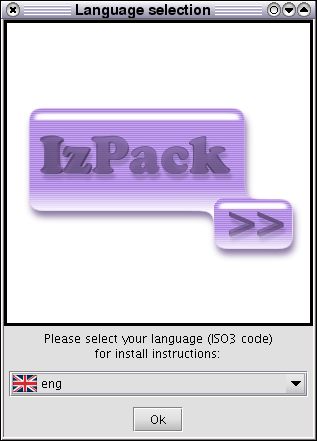
\includegraphics[scale=0.5]{img/lang-sel-splash}}
\IzPack is a tool that will help you to solve your software installation
problems. It is a \Java based software installer builder that will run
on any operating system coming with a \textit{Java Virtual Machine
(JVM)} that is compliant with the Sun JVM 1.2 or higher. Its design is
very modular and you will be able to choose how \textbf{you} want your
installer to look and you will also be able to customize it using a very
simple \textit{Application Programming Interface (API)}. Although
\IzPack is essentially a \Java only application (it can run on virtually
any operating system), it can interact in a clean way with the
underlying operating system. Native code can interact with it on a
specific platform without disturbing the operation on incompatible
operating systems. For instance, you can develop Unix-specific code that
will be silent if run on Windows. To put it in a nutshell, whereas most
of the other \Java installers force you to go their way, \IzPack will
let you go \textbf{your way}. Some respectable companies have been using
it in order to produce customized  installers for their \textsl{very}
specific needs.\\

\textit{"So, if it's so good, how much is it ?"} : well, you can get it
for free. \textbf{BUT} \IzPack is not a \textit{freeware}. It's not
\textit{free} as in \textit{"free beer"} but \textit{"free as in free
speech"}. So it's neither \textit{freeware} nor \textit{public domain}.
It is software covered by the \textsc{GNU General Public License} (GPL).
It uses the tactic of \textit{copyleft} : to make it short, you can use
it, modify it and redistribute it freely but you must also make your
modifications available to everyone whenever you publish a modified
version of a \textit{copylefted} software. You have access to the
\IzPack source code and you can modify it to make it suit your needs,
but if you publish such a modified version, you are forced to publish
the modifications you've made. \underline{That's a fair exchange of
expertise and  work}. To learn more about the GPL license and the
\textit{copyleft} principles, visit \mbox{\url{http://www.gnu.org/}}.\\

% Features
\section*{The Features}

\IzPack uses XML files to describe installations. When you make an
installer, you have a choice of panels. You can see panels as a kind of
plugin that composes the installer. For instance, a panel can choose the
installation path, the packs to install, prompt the user for a license
agreement and so on. This approach is very modular. You can also create
your own panels if you have specific needs. In some cases you even have
a choice from multiple panel versions for the same task. You can also
choose the order in which panels appear during the installation process.
\IzPack can be used in a number of different ways:
\begin{itemize}
  \item by writing the XML installation file "by hand" and compiling
  it with the command line compiler
  \item by invoking the compiler from the great \textsc{Apache Jakarta
  Ant} tool (see \url{http://jakarta.apache.org/}) as \IzPack can be
  used as a task for \textsc{Ant}
  \item by using the GUI based frontend. The frontend can be used to
  both generate the XML file and to initiate the compilation process.
\end{itemize}\

Here is a brief (and certainly incomplete !) list of the main \IzPack features :
\begin{itemize}
  \item XML based installation files
  \item easy internationalization using XML files (10 translations are already
  available)
  \item Ant integration, command-line compiler and GUI frontend
  \item easy customization with the panels and a rich API (even an XML parser is
  included !)
  \item powerful variable substitution system that you can use to customize
  scripts and more generally any text-based file
  \item different kinds of installers (standard, web-based, ...)
  \item launching of external executables during the installation process and Unix
  executable flag support (useful for the scripts for instance)
  \item layout of the installation files in packs (some can be optional)
  \item native code integration facilities
  \item jar files nesting support
  \item ... \textsl{more things to discover and create !}.
\end{itemize}\

% Development
\section*{The Development}

I started writing \IzPack in April 2001 and many people have helped me
improving it since. I prefer not to mention them here as I would for sure forget
some of them, so please check the file named \texttt{Thanks.txt} which I try to
get as up-to-date as possible in order to mention everyone who helped me. As far
as I'm concerned, I'm a french student and I rather see this as a fun activity
in my free time where I can learn a lot of great things. The contributors to the
project are both individuals and companies. Help can take any form :
\begin{itemize}
  \item translations
  \item new features and various fixes
  \item bug fixes
  \item writing manuals
  \item ... anything else you like :-)
\end{itemize}\

The official \IzPack homepage is located at
\mbox{\url{http://www.izforge.com/izpack/}}. There is a mailing-list available 
(\url{izpack.ml@izforge.com}) and you can subscribe to it by sending an email to
\url{izpack.ml_request@izforge.com} and typing \texttt{subscribe} in the 
subject field. Consider the mailing-list as the best way to get help about
IzPack and for submitting new ideas and contributions.\\

There are two types of releases for \IzPack :
\begin{itemize}
  \item a \textit{stable} release that is ready for production use
  \item an \textit{unstable} release that may contain bugs and incomplete
  features. This is the result of regular CVS snapshots.
\end{itemize}\

To access CVS, please use this \texttt{CVSROOT} :\\
\texttt{':pserver:anonymous@cvs.tuxfamily.org:/cvsroot/izpack2'}. A \textbf{BIG}
thank you to the TuxFamily team (see \url{http://www.tuxfamily.org/}). If you need
read/write access to contribute to \IzPack, then ask me at
\url{julien@izforge.com}. Of course don't forget to replace \texttt{'anonymous'}
for your login. There are two modules in CVS :
\begin{itemize}
  \item \texttt{izpack-src} : contains a minimal image that can be used to
  generate an installer for the \IzPack CVS version (if you need to use a
  CVS version then use the installed one, not the CVS files directly)
  \item \texttt{izpack-guidelines} : contains the \IzPack coding guidelines
  for those interessted in contributing to the project.
\end{itemize}\

% 3rd party used
\section*{3rd party code used in \IzPack}

\IzPack uses several 3rd party libraries and I would like to mention them in
respect for their respective authors work :
\begin{itemize}
  \item \textit{NanoXML} by Marc \textsc{De Scheemaecker} : the XML parser used
  inside \IzPack and released under a \textit{zlib/png}-style license - see\\
  \url{http://nanoxml.sourceforge.net/} -
  \item \textit{Kunststoff Look and Feel} by Incors Gmbh : a Swing\texttrademark 
  \ Look and Feel
  that can be used for installers. It \textbf{really} looks good and
  is released under the \textsc{GNU Lesser General Public License (LGPL)} - see
  \url{http://www.incors.org/} -
  \item \textit{Swing Connection Icons} : the icons used in \IzPack come from
  the \Java section of the Sun website - see \url{http://java.sun.com/} -
  \item \textit{Jakarta Ant DirectoryScanner class} : allows the use of Ant
  filesets syntax support. 
\end{itemize}\

So, now let's dive into understanding how \IzPack works. You'll be
surprised to see how powerful and simple it can be :-)

  % Chapter 1
\chapter{Getting started}

% Overview
\section{Overview}

To begin with, you should know what \IzPack is organized if you want to use
it. Let's go into the directory where you have installed \IzPack on your
machine. There are 3 text files and a set of directories. The most
important for the moment are \texttt{bin/ doc/ sample/}. If you are reading this,
you already know that \texttt{doc} contains this documentation :-)\\

So let's go into \texttt{bin/}. The \texttt{icons/} directory contains some
directories for your system, in case you would like an icon to launch a
component of \IzPack. But the most important things you can see in \texttt{bin}
are the \texttt{izpack-fe} and \texttt{compile} scripts (in both Unix* and
Windows formats). \texttt{izpack-fe} will launch the GUI based frontend of
\IzPack. It gives you the ability to prepare an installation XML file and
compile it to generate your installer. \texttt{compile} is used to compile a
ready-to-go XML installation file from a command-line context or from an
external tool.\\

\noindent
\textit{Note : these scripts can be launched from anywhere on your system as the
installer has customized these scripts so that they can inform \IzPack of where
it is located.}\\

% First Compilation
\section{First Compilation}

Now you probably can't wait to build your first installer. So go on open a
command-line shell and navigate to \texttt{sample/}. The following should work
on both Unix* and Windows systems. For the latter, just change the path
separator (slash '/') to a backslash. So type (\$ is your shell prompt !) :
\begin{verbatim}
$ ../bin/compile install.xml -b . -o install.jar -k standard
 (installer generation text output here)
$ java -jar install.jar
\end{verbatim}

There you are! The first command has produced the installer and the
second one did launch it. You can do the same thing by using the
frontend. You launch it with the \texttt{izpack-fe} script located in
\texttt{bin/}.\\

\fbox{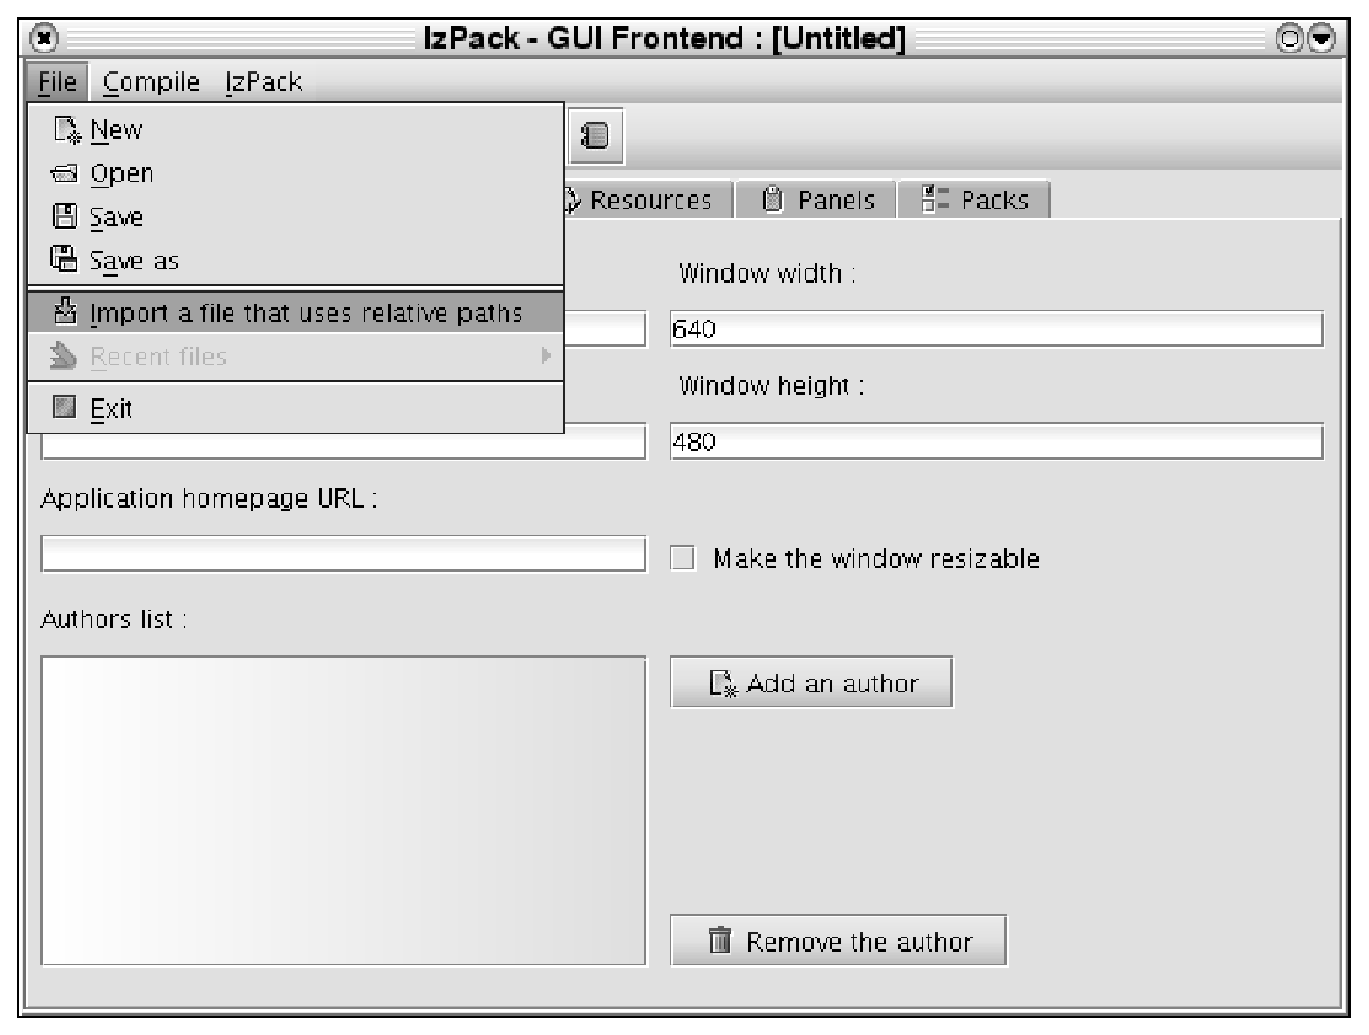
\includegraphics[scale=0.30]{img/ch1-import.eps}}Like on
the picture, import the file by selecting it from the \texttt{sample/}
directory. Then you will be asked for a base path, just go one directory
back and select \texttt{sample/}. The different fields of the frontend
should be filled properly. To compile the installer, just go into the
\textit{compile} menu and select a \textit{standard} kind of installer.
It will ask you for an output file name, just enter install.jar. The
building process should work just as smooth as in command-line mode.\\

% The IzPack Architecture
\section{The \IzPack Architecture}

Now that you have packaged your first installer, it's time for you to understand
how the whole thing works.\\

\subsection{The Compilation System}

The compilation system (see figure \ref{comparch}) is quite modular. 
Indeed, you can use the compiler in 3 ways :
\begin{itemize}
  \item from a command-line
  \item from the GUI frontend
  \item from Jakarta Ant
\end{itemize}\

\begin{figure}[h]
\caption{\label{comparch}
         \textit{The compiler architecture.}}
\begin{center}
\fbox{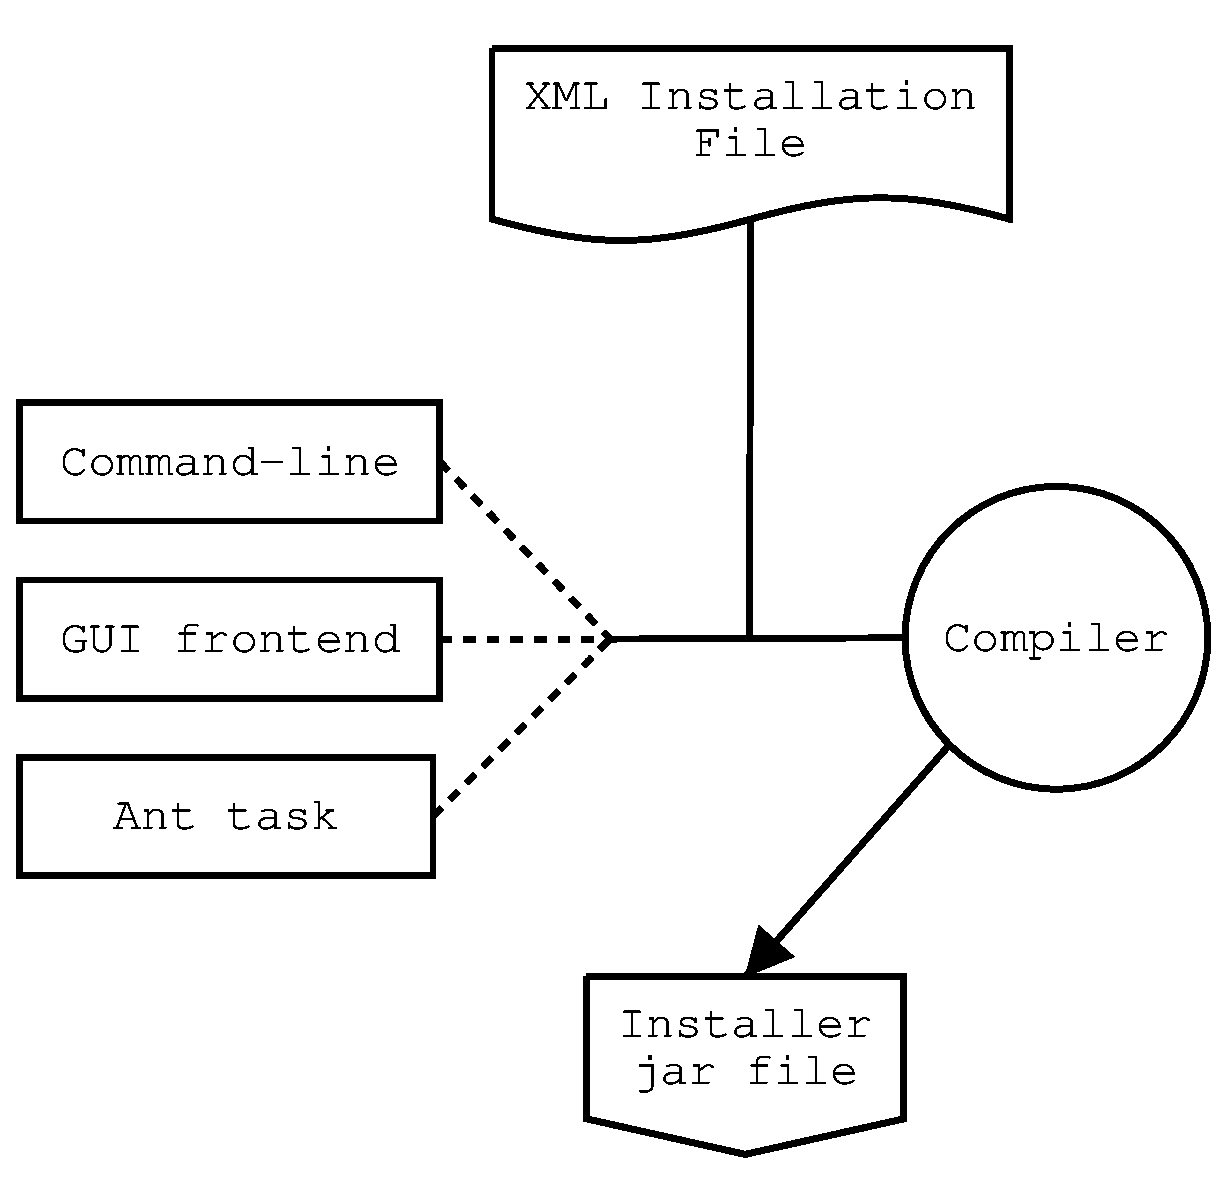
\includegraphics[scale=0.4]{img/ch1-comparch.eps}}
\end{center}
\end{figure}

The compiler takes as its input an XML installation file that describes
(at a relatively high-level) the installation. This file contains
detailed information such as the application name, the authors, the
files to install, the panels to use, which resources to load and much
more (see figure \ref{archinstaller}).\\

The compiler can generate different kinds of installers, but this information is
not located inside the XML file as it is not were it should be. On the contrary,
this is a compiler parameter.\\

\subsection{How an Installer Works}

An installer presents its panels to the end-user. For instance, there is
one to select the packages, one to prompt for the license agreement, one
to select the installation path and so on. You have a choice from a
variety of panels to place in the installer. For example, you can choose
between a plain text and a HTML text panel for the license agreement.
Also, if you don't want of the \textit{HelloPanel}, you just don't
include it.\\ 

\begin{figure}[h]
\caption{\label{archinstaller}
         \textit{The installer architecture.}}
\begin{center}
\fbox{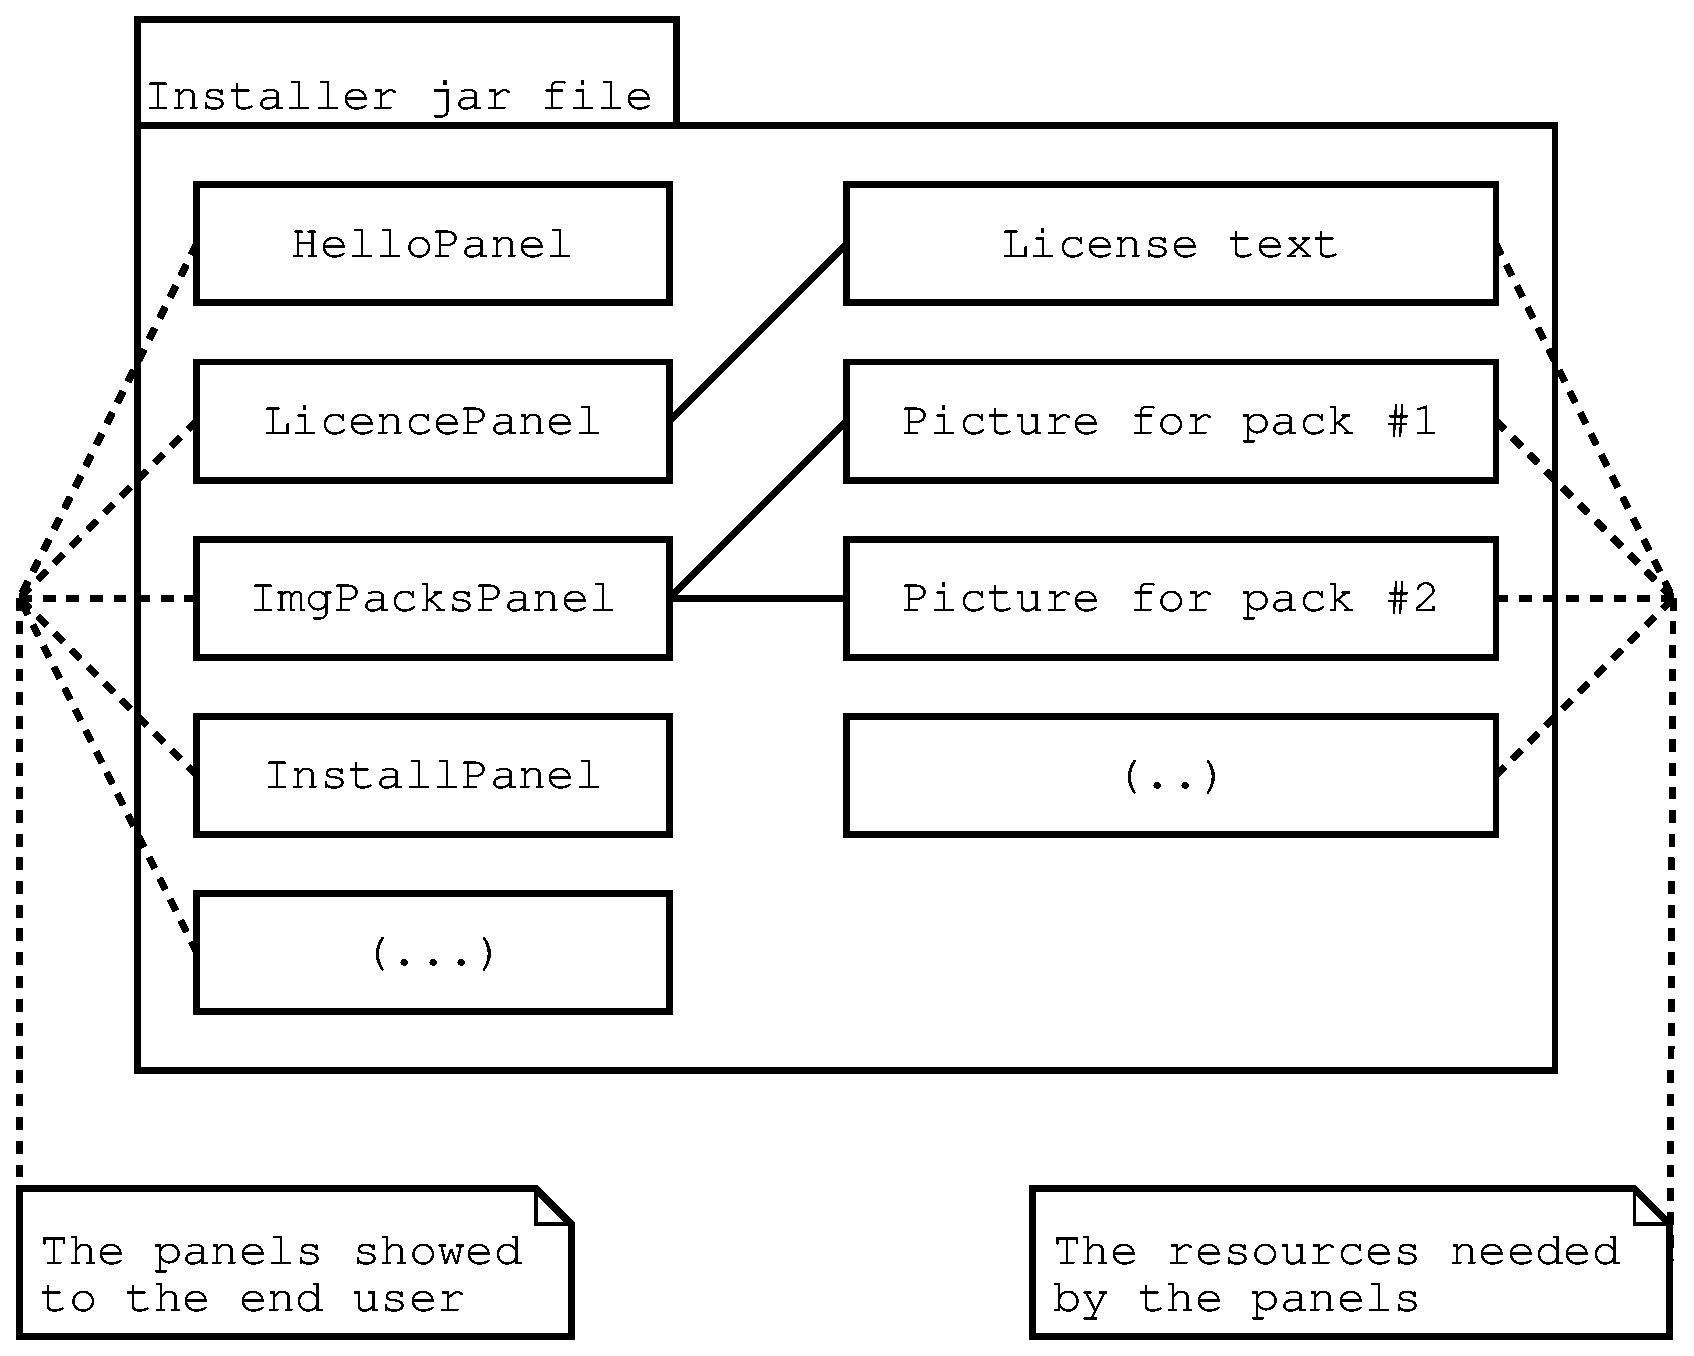
\includegraphics[scale=0.4]{img/ch1-compinside.eps}}
\end{center}
\end{figure}

It is very important to understand that some of the panels may need extra data. For
instance, the license agreement panel needs the license text. A simple approach
to specify such data would have been to add as many XML tags as needed for
each panel. However, this makes the XML file too specific and not easy to
maintain. The approach that has been chosen is to put the data in files and we
call these files \textit{resource files}. They are specified with a unique XML
tag. This is a much cleaner approach.\\

You might wonder how your files are packaged. They can be grouped in
\textit{packs}. For instance, you can have one pack for the core files, one for
the documentation, one for the source code and so one. In this way, your end-users
will have the choice to install a pack or not (provided that the pack they don't
want to install is not mandatory). Inside the jar file (which is a zip file), a
sub directory contains the pack files. Each pack file contains the files that are
part of it. Could we do it simpler ? :-)\\

\subsection{The Different Kinds of Installers}

There are for the moment 4 kinds of installers available :
\begin{itemize}

  \item \texttt{standard} : a single-file ready-to-run installer
  \item \texttt{standard-kunststoff} : same as above but using the Kunststoff
  Look and Feel
  \item \texttt{web} : a web based installer (the packs files are located on a
  HTTP server and the user installer will fetch it for him)
  \item \texttt{web-kunststoff} : same as above but using the Kunststoff
  Look and Feel.

\end{itemize}\

  % Chapter 2
\chapter{Writing Installation XML Files}

% What you need
\section{What You Need}

\subsection{Your editor}

In order to write your XML installation files, you just need a plain
text editor. Of course it's always easier to work with color coded text,
so you might rather want to work with a text editor having such a
feature. Here is a list of free editors that work well :
\begin{itemize}
  \item Jext : \url{http://www.jext.org/}
  \item JEdit : \url{http://www.jedit.org/}
  \item classics like Vim and (X)Emacs.
\end{itemize}\

\subsection{Writing XML}

Though you might not know much about XML, you have certainly heard about
it. If you know XML you can skip this subsection as we will briefly
present how to use XML.\\

XML is a markup language, really close to HTML. If you've ever worked
with HTML the transition will be fast. However there are a few little
things to know. The markups used in XML have the following form :
\texttt{<markup>}. Each markup has to be closed somewhere with its
ending tag : \texttt{</markup>}. Each tag can contain text and other
markups. If a markup does not contain anything, it is just reported once
: \texttt{<markup/>}. A markup can contain attributes like :
\texttt{<markup attr1="123" attr2="hello !"/>}. Here is a sample of a
valid XML structure :
\footnotesize
\begin{verbatim}
<chapter title="Chapter 1">
  <section name="Introduction">
    <paragraph>
    This is the text of the paragraph number 1. It is available for the very low
    price of <price currency="dollar">1 000 000</price>.
    </paragraph>
  </section>
  <section name="xxx">
  xxx
  </section>
</chapter>
\end{verbatim}
\normalsize

You should be aware of the following common mistakes :
\begin{itemize}

  \item markups \textbf{are} case sensitive : \texttt{<markup>} is different
  from \texttt{<Markup>}.
  
  \item you \textbf{must} close the markups in the same order as you create them
  : \texttt{<m1><m2>(...)</m2></m1>} is right but 
  \texttt{<m1><m2>(...)</m1></m2>} is not.

\end{itemize}

Also, an XML file must start with the following header :\\
\texttt{<?xml version="1.0" encoding="iso-8859-1 standalone="yes" ?>}. The only
thing you should modify is the encoding (put here the one your text editor saves
your files to). The \texttt{standalone} attribute is not very important for
us.\\

This (brief !) introduction to XML was just meant to enable you to write
your installation specification. For a better introduction there are
plenty of books and articles/tutorials dealing with XML on the Internet,
in book stores, in magazines and so on.\\

% Built-in variables
\section{Variable Substitution}

During the installation process IzPack can substitute variables in
various places with real values. Obvious targets for variable
substitution are resource files and launch scripts, however you will
notice many more places where it is more powerful to use variables
rather then hard coded values. Wherever variables can be used it will
be explained in the documentation.\\

There are two types of variables:
\begin{itemize}
  \item Built-In variables. These are implemented in IzPack and are 
        all dynamic in nature. This means that the value of each
        variable depends on local conditions on the target system.
  \item Variables that you can define. You also define the value,
        which is fixed for a given installation file.
\end{itemize}

You define your own variables in the installation XML file with the
\texttt{<variable>} tag. How to do this is explained in detail later in
this chapter.\\

\textbf{Please note} that when using variables they must always appear
with a '\texttt{\$}' sign as the first character, even though they are
not defined this way.\\

\subsection{The Built-In Variables}
The following variables are built-in :
\begin{itemize}
  \item \texttt{\$INSTALL\_PATH} : the installation path on the
        target system, as chosen by the user
  \item \texttt{\$JAVA\_HOME} : the \Java virtual machine home path
  \item \texttt{\$USER\_HOME} : the user's home directory path
  \item \texttt{\$USER\_NAME} : the user name
  \item \texttt{\$APP\_NAME} : the application name
  \item \texttt{\$APP\_URL} : the application URL
  \item \texttt{\$APP\_VER} : the application version
  \item \texttt{\$ISO3\_LANG} : the ISO3 language code of the selected langpack.
\end{itemize}\

\subsection{Parse Types}
Parse types apply only when replacing variables in text files. At places
where it might be necessary to specify a parse type, the documentation
will mention this. Depending on the parse type, IzPack will handle
special cases -such as escaping control characters- correctly. The
following parse types are available:
\begin{itemize}
  \item \texttt{plain} - use this type for plain text files, where no
        special substitution rules apply. All variables will be
        replaced with their respective values as is.
  \item \texttt{javaprop} - use this type if the substitution happens
        in a Java properties file. Individual variables might be
        modified to function properly within the context of Java
        property files.
  \item \texttt{xml} - use this type if the substitution happens in
        a XML file. Individual variables might be modified to function
        properly within the context of XML files.
  \item \texttt{shell} - use this type if the substitution happens in
        a shell script. Because shell scripts use \texttt{\$variable} 
        themselves, an alternative variable marker is used: 
        \texttt{\%variable} or \texttt{\%\{variable\}}.
\end{itemize}

% The IzPack elements
\section{The \IzPack Elements}

\noindent
\textit{When writing your installer XML files, it's a good idea to have a look
at the \IzPack installation DTD}.\\

\subsection{The Root Element \texttt{<installation>}}
\label{root-element}

The root element of an installation is \texttt{<installation>}. It takes
one required attribute : \texttt{version}. The attribute defines the
version of the XML file layout and is used by the compiler to identify
if it is compatible with the XML file. This should be set to $1.0$ for
the moment.\\

\subsection{The Information Element \texttt{<info>}}
\label{info-element}

This element is used to specify some general information for the installer. It
contains the following elements :
\begin{itemize}

  \item \texttt{<appname>} : the application name
  \item \texttt{<appversion>} : the application version
  \item \texttt{<url>} : the application official website url
  \item \texttt{<authors>} : specifies the author(s) of the application. It must contain
  at least one \texttt{<author>} element whose attributes are :
  \begin{itemize}
    \item \texttt{name} : the author's name
    \item \texttt{email} : the author's email
  \end{itemize}
  \item \texttt{<uninstaller>} : specifies whether to create an uninstaller after installation, it has only the \texttt{write} attribute, with default value \texttt{yes}. If this tag is not specified, the uninstaller will still be written.
  \item \texttt{<javaversion>} : specifies the minimum version of Java required to install your program. Values can be \texttt{1.2}, \texttt{1.2.2}, \texttt{1.4}, etc. The test is a lexical comparison against the \texttt{java.version} System property on the install machine.
  \item \texttt{<webdir>} : Causes a ``web installer'' to be created, and specifies the URL packages are retrieved from at install time. The content of the tag must be a properly formed URL. See section~\ref{webinstaller} for more details.

\end{itemize}\

Here is an example of a typical \texttt{<info>} section :\\
\footnotesize
\begin{verbatim}
<info>
  <appname>Super extractor</appname>
  <appversion>2.1 beta 6</appversion>
  <url>http://www.superextractor.com/</url>
  <authors>
    <author name="John John Doo" email="jjd@jjd-mail.com"/>
    <author name="El Goyo" email="goyoman@mymail.org"/>
  </authors>
  <javaversion>1.2</javaversion>
</info>
\end{verbatim}
\normalsize

\subsection{The Variables Element \texttt{<variables>}}
\label{variables-element}

This element allows you to define variables for the variables
substitution system. Some variables are built-in, such as
\texttt{\$INSTALL\_PATH} (which is the installation path chosen by the
user). When you define a set of variables, you just have to place as
many \texttt{<variable>} tags in the file as needed. If you define a
variable named \texttt{VERSION} you need to type \$VERSION in the files
to parse. The variable substitutor will then replace it with the correct
value. One \texttt{<variable>} tag take the following attributes :
\begin{itemize}

  \item \texttt{name} : the variable name
  \item \texttt{value} : the variable value

\end{itemize}\

Here's a sample \texttt{<variables>} section :\\
\footnotesize
\begin{verbatim}
<variables>
  <variable name="app-version" value="1.4"/>
  <variable name="released-on" value="08/03/2002"/>
</variables>
\end{verbatim}
\normalsize

\subsection{The GUI Preferences Element \texttt{<guiprefs>}}
\label{guiprefs-element}

This element allows you to set the behavior of your installer GUI. This
information will not have any effect on the command-line installers that will be
available in future versions of \IzPack. The arguments to specify are :
\begin{itemize}

  \item \texttt{resizable} : takes \texttt{yes} or \texttt{no} and indicates
  whether the window size can be changed or not.
  \item \texttt{width} : sets the initial window width
  \item \texttt{height} : sets the initial window height.
  
\end{itemize}\

Here's a sample :
\footnotesize
\begin{verbatim}
<guiprefs resizable="no" width="800" height="600"/>
\end{verbatim}
\normalsize

Starting from IzPack 3.6, the look and feel can be specified in this section on
a per-OS basis. For instance you can use the native look and feels on Win32 and
OS X but use a third-party one on Unix-like platforms. To do that, you have to
add some children to the \texttt{guiprefs} tag:
\begin{itemize}

  \item \texttt{laf}: the tag that specifies a look and feel. It has a
  \texttt{name} parameter that defines the look and feel name.
  \item Each \texttt{laf} element needs at least one \texttt{os} tag, specified
  like in the other parts of the specification that support this tag.
  \item Like you can add \texttt{os} elements, you can add any number of
  \texttt{param} elements to customize a look and feel. A \texttt{param}
  elements has two attribues: \texttt{name} and \texttt{value}.

\end{itemize}\

The available look and feels are:
\begin{itemize}

  \item Kunststoff: \texttt{kunststoff}
  \item Liquid: \texttt{liquid}
  \item Metouia: \texttt{metouia}
  \item JGoodies Looks: \texttt{looks}

\end{itemize}\

If you don't specify a look and feel for a particular operating system, then the
default native one will be used: Windows on Windows, Aqua on Mac OS X and Metal
on the Unix-like variants.\\

The \textit{Liquid Look and Feel} supports the following parameters:
\begin{itemize}

  \item \texttt{decorate.frames}: \texttt{yes} means that it will render the
  frames in Liquid style
  \item \texttt{decorate.dialogs}: \texttt{yes} means that it will render the
  dialogs in Liquid style

\end{itemize}\

The \textit{JGoodies Looks} look and feel can be specified by using the
\texttt{variant} parameters. The values can be one of:
\begin{itemize}

  \item \texttt{extwin}: use the Windows Extension look
  \item \texttt{plastic}: use the basic Plastic look
  \item \texttt{plastic3D}: use the Plastic 3D look
  \item \texttt{plasticXP}: use the Plastic XP look (default).

\end{itemize}\

Here is a small sample:
\begin{verbatim}
<guiprefs height="600" resizable="yes" width="800">
    <laf name="metouia">
        <os family="unix" />
    </laf>
    <laf name="looks">
        <os family="windows" />
        <param name="variant" value="extwin" />
    </laf>
</guiprefs>
\end{verbatim}

\subsection{The Localization Element \texttt{<locale>}}
\label{localization-element}

This element is used to specify the language packs (langpacks) that you want to
use for your installer. You must set one \texttt{<langpack>} markup per
language. This markup takes the \texttt{iso3} parameter which specifies the iso3
language code.\\

Here's a sample :\\
\footnotesize
\begin{verbatim}
<locale>
  <langpack iso3="eng"/>
  <langpack iso3="fra"/>
  <langpack iso3="spa"/>
</locale>
\end{verbatim}\
\normalsize

The supported ISO3 codes are :
\begin{center}
\begin{tabular}{|l|l|}
\hline
\textit{ISO3 code} & \textit{Language} \\ \hline
cat & Catalunyan \\ \hline
dan & Danish \\ \hline
deu & German \\ \hline
eng & English \\ \hline
fin & Finnish \\ \hline
fra & French \\ \hline
hun & Hungarian \\ \hline
ita & Italian \\ \hline
jpn & Japanese \\ \hline
mys & Malaysian \\ \hline
ned & Nederlands \\ \hline
pol & Polnish \\ \hline
por & Portuguese (Brazilian) \\ \hline
rom & Romanian \\ \hline
rus & Russian \\ \hline
spa & Spanish \\ \hline
svk & Slovakian \\ \hline
swe & Swedish \\ \hline
ukr & Ukrainian \\ \hline
\end{tabular}\
\end{center}

\subsection{The Resources Element \texttt{<resources>}}
\label{resources-element}

Several panels, such as the license panel and the shortcut panel,
require additional data to perform their task. This data is supplied
in the form of resources. This section describes how to specify
them. Take a look at each panel description to see if it might need
any resources. Currently, no checks are made to ensure resources
needed by any panel have been included. The \texttt{<resources>}
element is not required, and no \texttt{<res>} elements are required
within.\\

You have to set one \texttt{<res>} markup for each resource. Here are
the attributes to specify :
\begin{itemize}

  \item \texttt{src} : the path to the resource file which can be named freely
  of course (for instance \texttt{my-picture.jpg}).
  \item \texttt{id} : the resource id, depending on the needs of a particular panel
  \item \texttt{parse} : takes \texttt{yes} or \texttt{no} (default is
  \texttt{no}) - used to specify whether the resource must be parsed at the
  installer compilation time. For instance you could set the application version
  in a readme file used by \texttt{InfoPanel}.
  \item \texttt{type} : specifies the parse type. This makes sense only for a text
  resource  - the default is \texttt{plain}, other values are \texttt{javaprop,
  xml} (Java properties file and XML files)
  \item \texttt{encoding} : specifies the resource encoding if the receiver needs
  to know. This makes sense only for a text resource.

\end{itemize}\

Here's a sample :
\footnotesize
\begin{verbatim}
<resources>
  <res id="InfoPanel.info" src="doc/readme.txt" parse="yes"/>
  <res id="LicencePanel.licence" src="legal/License.txt"/>
</resources>
\end{verbatim}
\normalsize

\subsection{The Panels Element \texttt{<panels>}}
\label{panels-element}

Here you tell the compiler which panels you want to use. They will
appear in the installer in the order in which they are listed in your
XML installation file. Take a look at the different panels in order to
find the ones you need. The \texttt{<panel>} markup takes a single
attribute \texttt{classname} which is the classname of the panel.\\

Here's a sample :
\footnotesize
\begin{verbatim}
<panels>
  <panel classname="HelloPanel"/>
  <panel classname="LicencePanel"/>
  <panel classname="TargetPanel"/>
  <panel classname="InstallPanel"/>
  <panel classname="FinishPanel"/>
</panels>
\end{verbatim}
\normalsize

\subsection{The Packs Element \texttt{<packs>}}
\label{packs-element}

This is a crucial section as it is used to specify the files that need
to be installed. The \texttt{<packs>} section consists of several 
\texttt{<pack>} tags.

The \texttt{<pack>} takes the following attributes :
  \begin{itemize}
    \item \texttt{name}: the pack name
    \item \texttt{required}: takes \texttt{yes} or \texttt{no} and specifies
    whether the pack is optional or not.
    \item \texttt{os}: optional attribute that lets you make the pack targeted
    to a specific \textsl{operating system}, for instance \texttt{unix},
    \texttt{mac} and so on.
    \item \texttt{preselected}: optional attribute that lets you choose whether
    the pack is by default selected for installation or not. Possible values
    are \texttt{yes} and \texttt{no}. A pack which is not preselected needs to
    be explicitly selected by the user during installation to get installed.
    \item \texttt{loose}: can be used so that the files are not located in the
    installer Jar. The possible values are \texttt{true} or \texttt{false}, the
    default beeing \texttt{false}. The author of this feature needed to put his
    application on a CD so that the users could run it directly from this media.
    However, he also wanted to offer them the possibility to install the
    software localy. Enabling this feature will make IzPack take the files on
    disk instead of from the installer. \textit{Please make sure that your relative
    files paths are correct !}
    \item \texttt{id}: this attribute is used to give a unique id to the pack to
    be used for internationalization.
  \end{itemize}

\subsubsection{Internationalization of the PacksPanel}
In order to provide internationalization for the PacksPanel, so that your users can
be presented with a different name and description for each language you support,
 you have to create a file named \texttt{packsLang.xml\_xyz} where \texttt{xyz}
 is the ISO3 code of the language in lowercase. Please be aware that case is significant.
 This file has to be inserted in the resources section of \texttt{install.xml} with the
 \texttt{id} and \texttt{src} attributes set at the name of the file. The format of
 these files is identical with the distribution langpack files located at
 \texttt{\$IZPACK\_HOME/install/langpacks/installer}. For the name of the panel you just
 use the pack \texttt{id} as the txt \texttt{id}. For the description you use the pack
 \texttt{id} suffixed with \texttt{'.description'}.

The following sections describe the tags available for a \texttt{<pack>} section.

\subsubsection{\texttt{<description>} - pack description}

The contents of the \texttt{<description>} tag describe the pack contents.
This description is displayed if the user highlights the pack during 
installation.

\subsubsection{\texttt{<depends>} - pack dependencies}
This can be used to make this pack selectable only to be installed only if some other is 
selected to be installed. The pack can depend on more than one by specifying more than one
\texttt{<depends>} elements.\\ 
Circular depedencies are not supported and the compiler reports an error if one occurs.

This tag takes the following attribute:
\begin{itemize}
\item \texttt{packname}: The name of the pack that it depends on
\end{itemize}

\subsubsection{\texttt{<os>} - OS restrictions}

It is possible to restrict a panel to a certain list of operating systems. This
tag takes the following attributes:
\begin{itemize}
\item \texttt{family}: unix, windows or mac
\item \texttt{name}: the exact OS name (ie Windows, Linux, ...)
\item \texttt{version}: the exact OS version (see the JVM \texttt{os.version} property)
\item \texttt{arch}: the machine architecture (see the JVM \texttt{os.arch} property).
\end{itemize}

\subsubsection{\texttt{<updatecheck>}}

This feature can update an already installed package, therefore removing
superfluous files after installation. Here's how this feature author (Tino Schwarze)
described it on the IzPack development mailing-list:
\begin{quote}
Each pack can now
specify an \texttt{<updatecheck>} tag. It supports a subset of ant fileset
syntax, e.g.:
\begin{verbatim}
<updatecheck>
  <include name="lib/**" />
  <exclude name="config/local/** />
</updatecheck>
\end{verbatim}\

If the paths are relative, they will be matched relative to
\texttt{\$INSTALL\_PATH}. Update checks are only enabled if at least one
\texttt{<include>} is specified. See
\texttt{com.izforge.izpack.installer.Unpacker} for details.
\end{quote}

\subsubsection{\label{tag:file}\texttt{<file>} - add files or directories}

The \texttt{<file>} tag specifies a file (a directory is a file too) to 
include into the pack. It takes the following attributes:

\begin{itemize}

  \item \texttt{src}: the file location (relative path) - if this is a
  directory its content will be added recursively

  \item \texttt{targetdir}: the destination directory, could be something like
  \texttt{\$INSTALL\_PATH/subdirX}

  \item \texttt{os}: can optionally specify a target operating system
  (\texttt{unix, windows, mac}) - this means that the file will only be
  installed on its target operating system

  \item \texttt{override}: if \texttt{true} then if the file is already
  installed, it will be overwritten. Alternative values: \texttt{asktrue} and
  \texttt{askfalse} -- ask the user what to do and supply default value for
  non-interactive use. Another possible values is \texttt{update}. It means
  that the new file is only installed if it's modification time is newer than
  the modification time of the already existing file (note that this is not a
  reliable mechanism for updates - you cannot detect whether a file was
  altered after installation this way.) By default it is set to \texttt{update}.

\end{itemize}
\paragraph{\label{tag:additionaldata}\texttt{<additionaldata>}}

This tag can also be specified in order to pass additional data
related to a file tag for customizing.

\begin{itemize}

  \item \texttt{<key>}: key to identify the data
  \item \texttt{<value>}: value which can be used by a custom
  action

\end{itemize}

\subsubsection{\label{tag:singlefile}\texttt{<singlefile>} - add a single file}

Specifies a single file to include. The difference to \texttt{<file>} is that
this tag allows the file to be renamed, therefore it has a 
\texttt{target} attribute instead of \texttt{targetdir}.

\begin{itemize}

  \item \texttt{src}: the file location (relative path)

  \item \texttt{target}: the destination file name, could be something
  like \texttt{\$INSTALL\_PATH/subdirX/fileY}

  \item \texttt{os}: can optionally specify a target operating system
  (\texttt{unix, windows, mac}) - this means that the file will only be
  installed on its target operating system

  \item \texttt{override}: see \texttt{<file>} (\ref{tag:file}) for description

\end{itemize}
A \texttt{<additionaldata>} (\ref{tag:additionaldata}) tag can
also be specified for customizing.

\subsubsection{\label{tag:fileset}\texttt{<fileset>}: add a fileset}

The \texttt{<fileset>} tag allows files to be specified using the powerful
Jakarta Ant set syntax. It takes the following parameters:

\begin{itemize}

  \item \texttt{dir}: the base directory for the fileset (relative path)

  \item \texttt{targetdir}: the destination path, works like for
  \texttt{<file>}

  \item \texttt{casesensitive}: optionally lets you specify if the names
  are case-sensitive or not - takes \texttt{yes} or \texttt{no}

  \item \texttt{defaultexcludes}: optionally lets you specify if the default
  excludes will be used - takes \texttt{yes} or \texttt{no}.

  \item \texttt{os}: specifies the operating system, works like for
  \texttt{<file>}

  \item \texttt{override}: see \texttt{<file>} for description

  \item \texttt{includes}: comma- or space-separated list of patterns of
  files that must be included; all files are included when omitted.
  This is an alternative for multiple include tags.

  \item \texttt{excludes}: comma- or space-separated list of patterns of
  files that must be excluded; no files (except default excludes) are
  excluded when omitted. This is an alternative for multiple exclude tags.

\end{itemize}

You specify the files with  \texttt{<include>} and \texttt{<exclude>} tags
that take the \texttt{name} parameter to specify the Ant-like pattern :
\begin{itemize}    
  \item \texttt{**} : means any subdirectory
  \item \texttt{*} : used as a wildcard.
\end{itemize}
Here are some examples of Ant patterns :
\begin{itemize}

  \item \texttt{<include name="lib"/>} : will include \texttt{lib} and the
  subdirectories of \texttt{lib}

  \item \texttt{<exclude name="**/*.java"/>} : will exclude any file in any
  directory starting from the base path ending by \texttt{.java}

  \item \texttt{<include name="lib/*.jar"/>} : will include all the files
  ending by \texttt{.jar} in \texttt{lib}

  \item \texttt{<exclude name="lib/**/*FOO*"/>} : will exclude any file in
  any subdirectory starting from \texttt{lib} whose name contains
  \texttt{FOO}.

\end{itemize}

There area set of definitions that are excluded by default file-sets,
just as in Ant. IzPack defaults to the Ant list of default
excludes. There is currently no equivalent to the <defaultexcludes>
task. Default excludes are:
\footnotesize
\begin{verbatim}
     **/*\~{}
     **/\#*\#
     **/.\#*
     **/%*%
     **/.\_*
     **/CVS
     **/CVS/**
     **/.cvsignore
     **/SCCS
     **/SCCS/**
     **/vssver.scc
     **/.svn
     **/.svn/**
     **/.DS\_Store
\end{verbatim}
\normalsize
A \texttt{<additionaldata>} (\ref{tag:additionaldata})
tag can also be specified for customizing.

\subsubsection{\texttt{<parsable>} - parse a file after installation}

Files specified by \texttt{<parsable>} are parsed after installation and may
have variables substituted.

\begin{itemize}

  \item \texttt{targetfile} : the file to parse, could be something like\\
  \texttt{\$INSTALL\_PATH/bin/launch-script.sh}\\
  \label{tag:slashMasking}A slash will be changed to the system dependant path separator (e.g. to
  a backslash on Windows) only if no backslash masks the slash.

  \item \texttt{type} : specifies the type (same as for the resources) -
  the default is \texttt{plain}

  \item \texttt{encoding} : specifies the file encoding

  \item \texttt{os}: specifies the operating system, works like for
  \texttt{<file>}

\end{itemize}\

\subsubsection{\texttt{<executable>} - mark file executable or execute it}

The \texttt{<executable>} tag is a very useful thing if you need to execute
something during the installation process. It can also be used to set the
executable flag on Unix-like systems. Here are the attributes :

\begin{itemize}

  \item \texttt{targetfile} : the file to run, could be something like\\
  \texttt{\$INSTALL\_PATH/bin/launch-script.sh}\\
  Slashes are handled special (see attribute 
  \texttt{targetfile} of tag \texttt{<parsable>}\ref{tag:slashMasking}).

  \item \texttt{class} : If the executable is a jar file, this is the
  class to run for a \Java program

  \item \texttt{type} : \texttt{bin} or \texttt{jar} (the default is
  \texttt{bin})

  \item \texttt{stage} : specifies when to launch : \texttt{postinstall}
  is just after the installation is done and the default value,
  \texttt{never} will never launch it (useful to set the +x flag on Unix).
  \texttt{uninstall} will launch the executable when the application
  is uninstalled. The executable is executed before any files are deleted.

  \item \texttt{failure} : specifies what to do when an error occurs :
  \texttt{abort} will abort the installation process, \texttt{ask} (default)
  will ask the user what to do and \texttt{warn} will just tell the user
  that something is wrong

  \item \texttt{os}: specifies the operating system, works like for
  \texttt{<file>}

  \item \texttt{keep} : specifies whether the file will be kept after
  execution. The default is to delete the file after is has been executed.
  This can be changed by specifying \texttt{keep="true"}.

\end{itemize}
A \texttt{<args>} tag can also be specified in order to pass
arguments to the executable:
\begin{itemize}

  \item \texttt{<arg>}: passes the argument specified in the
  \texttt{value} attribute.   Slashes are handled special (see attribute 
  \texttt{targetfile} of tag \texttt{<parsable>}\ref{tag:slashMasking}).

\end{itemize}
  
\subsubsection{\label{tag:os}\texttt{<os>} - make a file OS-dependent}

The \texttt{<os>} tag can be used inside the \texttt{<file>},
\texttt{<fileset>}, \texttt{<singlefile>}, \texttt{<parsable>},
\texttt{<executable>} tags to restrict it's effect to a specific
operating system family, architecture or version:

\begin{itemize}

  \item \texttt{family}: \texttt{unix, windows, mac} to specify the
  operating system family
  \item \texttt{name}: the operating system name
  \item \texttt{version}: the operating system version
  \item \texttt{arch}: the operating system architecture (for instance the
  Linux kernel can run on i386, sparc, and so on)

\end{itemize}


Here's an example installation file :
\footnotesize
\begin{verbatim}
<packs>
    <!-- The core files -->
    <pack name="Core" required="yes">
        <description>The IzPack core files.</description>
        <file targetdir="$INSTALL_PATH" src="bin"/>
        <file targetdir="$INSTALL_PATH" src="lib"/>
        <file targetdir="$INSTALL_PATH" src="legal"/>
        <file targetdir="$INSTALL_PATH" src="Readme.txt"/>
        <file targetdir="$INSTALL_PATH" src="Versions.txt"/>
        <file targetdir="$INSTALL_PATH" src="Thanks.txt"/>
        <parsable targetfile="$INSTALL_PATH/bin/izpack-fe"/>
        <parsable targetfile="$INSTALL_PATH/bin/izpack-fe.bat"/>
        <parsable targetfile="$INSTALL_PATH/bin/compile"/>
        <parsable targetfile="$INSTALL_PATH/bin/compile.bat"/>
        <executable targetfile="$INSTALL_PATH/bin/compile" stage="never"/>
        <executable targetfile="$INSTALL_PATH/bin/izpack-fe" stage="never"/>
    </pack>
    
    <!-- The documentation (1 directory) -->
    <pack name="Documentation" required="no">
        <description>The IzPack documentation (HTML and PDF).</description>
        <file targetdir="$INSTALL_PATH" src="doc"/>
    </pack>
</packs>
\end{verbatim}
\normalsize

\subsection{The Native Element \texttt{<native>}}
\label{native-element}

Use this if you want to use a feature that requires a native library.
The native libraries are placed under \texttt{bin/native/..}. There are 2
kinds of native libraries : the \IzPack libraries and the third-party
ones. The IzPack libraries are located at \texttt{bin/native/izpack},
you can place your own libraries at \texttt{bin/native/3rdparty}. 
It is possible to place a native library also into the uninstaller. 
It is useable from CustomActions (\ref{cha:customactions}). If one or 
more are referenced for it, the needed support classes are automatically
placed into the uninstaller. To place it only on operating systems
for which they are build, it is possible to define an OS
restriction. This restriction will only be performed for the
uninstaller. The markup takes the following attributes :\begin{itemize}

  \item \texttt{type} : \texttt{izpack} or \texttt{3rdparty}
  \item \texttt{name} : the library filename
  \item \texttt{stage}: stage where to use the library
  (install|uninstall|both)

\end{itemize}\
\subsubsection{\texttt{<os>} - make a library OS-dependent}

The \texttt{<os>} tag can be used to restrict the inclusion into
the uninstaller to a specific operating system family,
architecture or version. The inclusion into the installer will be
always done. For more information see \ref{tag:os}.

Here's a sample :
\footnotesize
\begin{verbatim}
<native type="izpack" name="ShellLink.dll"/>
\end{verbatim}
\normalsize

\subsection{The Jar Merging Element \texttt{<jar>}}
\label{jar-element}

If you adapt \IzPack for your own needs, you might need to merge the
content of another jar file into the jar installer. For instance, this
could be a library that you need to merge. The \texttt{<jar>} markup
allows you to merge the raw content of another jar file into the 
installer and the uninstaller. It is necessary that the paths in the
jars are unique because only the contained files of the jar are added
to the installer jar, not the jar file self.
The attributes are:\begin{itemize}
\item \texttt{src} : the path at compile time
\item \texttt{stage}: stage where to use the contents of the additional jar file
  (install|uninstall|both)

\end{itemize}\


A sample :
\footnotesize
\begin{verbatim}
<jar src="../nicelibrary.jar"/>
\end{verbatim}
\normalsize

% The panels
\section{The Available Panels}

In this section I will introduce the various panels available in IzPack.
The usage for most is pretty simple and described right here. The more
elaborate ones are explained in more detail in the \textit{Advanced
Features} chapter or in their own chapter. The panels are listed by
their class name. This is the name that must be used with the
\texttt{classname} attribute (case-sensitive).\\

\subsection{HelloPanel}

This panel welcomes the user by displaying the project name, the
version, the URL as well as the authors.\\

\subsection{InfoPanel and HTMLInfoPanel}

This is a kind of 'README' panel. It presents text of any length. The
text is specified by the \texttt{(HTML)InfoPanel.info} resource. Starting from
IzPack 3.7.0, variables substitution is allowed.\\

\subsection{LicencePanel and HTMLLicencePanel}

\noindent
\textit{\underline{Note :} there is a mistake in the name - it should be
LicensePanel. In France the word is Licence ... and one of my diploma is a
'Licence' so ...} :-)\\

These panels can prompt the user to acknowledge a license agreement. They block
unless the user selects the 'agree' option. To specify the license agreement
text you have to use the \texttt{(HTML)LicencePanel.licence} resource.\\

\subsection{PacksPanel}

Allows the user to select the packs he wants to install.\\

\subsection{ImgPacksPanel}

This is the same as above, but for each panel a different picture is
shown to the user. The pictures are specified with the resources
\texttt{ImgPacksPanel.img.x} where x stands for the pack number, the
numbers start from 0. Of course it's up to you to specify as many images
as needed and with correct numbers. For instance if you have 2 packs
\texttt{core} and \texttt{documentation} (in this order), then the resource for
\texttt{core} will be \texttt{ImgPacksPanel.img.0} and the resource for
\texttt{doc} will be \texttt{ImgPacksPanel.img.1}. The supported image formats
depend on what you JVM supports, but starting from J2SE 1.3, \textsl{GIF},
\textsl{JPEG} and \textsl{PNG} are supported.\\

\subsection{TargetPanel}

This panel allows the user to select the installation path. It can be customized with
the following resources (they are text files containing the path) :
\begin{itemize}

  \item \texttt{TargetPanel.dir.f} where f stands for the family (\texttt{mac,
  macosx, windows, unix})
  \item \texttt{TargetPanel.dir} : the directory name, instead of the software
  to install name
  \item \texttt{TargetPanel.dir.d} where d is a "dynamic" name, as returned by
  the \Java virtual machine. You should write the name in lowercase and replace the
  spaces with underscores. For instance, you might want a different setting for
  Solaris and GNU/Linux which are both Unix-like systems. The resources would be
  \texttt{TargetPanel.dir.sunos, TargetPanel.dir.linux}. You should have a
  Unix-resource in case it wouldn't work though.

\end{itemize}\

\subsection{InstallPanel}

You should always have this one as it launches the installation process !\\

\subsection{XInfoPanel}

A panel showing text parsed by the variable substitutor. The text can be
specified through the \texttt{XInfoPanel.info} resource. This panel can
be useful when you have to show information after the installation
process is completed (for instance if the text contains the target
path).\\

\subsection{FinishPanel}

A ending panel, able to write automated installer information. For
details see the chapter on 'Advanced Features'.\\ 

\subsection{SimpleFinishPanel}

Same as \texttt{FinishPanel}, but without the automated installer features. It
is aimed at making the life easier for end-users who will never encounter the
automated installer extra feature.\\

\subsection{ShortcutPanel}

This panel is used to create desktop shortcuts. For details on using the
ShortcutPanel see the chapter 'Desktop Shortcuts'.

\subsection{UserInputPanel}

This panel allows you to prompt the user for data. What the user is prompted
for is specified using an XML file which is included as a resource to the
installer. See chapter \ref{chap:userinput} on page \pageref{chap:userinput}
for a detailed explanation.

\subsection{CompilePanel}

This panel allows you to compile just installed Java sourcecode. 
The details for the compilation are specified using the resource \texttt{CompilePanel.Spec.xml}.
The XML file has the following format:
\begin{verbatim}
<compilation>
  <global>
    <compiler>
      <choice value="$JAVA_HOME/bin/javac" />
      <choice value="jikes" />
    </compiler>
    <arguments>
      <choice value="-O -g:none" />
      <choice value="-O" />
      <choice value="-g" />
      <choice value="" />
    </arguments>
  </global>
  <jobs>
    <classpath add="$INSTALL_PATH/src/classes/" />
    <job name="optional name">
      <directory name="$INSTALL_PATH/src/classes/xyz" />
    </job>
    <job name="another job">
      <packdepency name="some package name" />
      <classpath sub="$INSTALL_PATH/" />
      <directory name="$INSTALL_PATH/src/classes/abc" />
      <file name="$INSTALL_PATH/some/file.java" />
    </job>
  </jobs>
</compilation>
\end{verbatim}

In theory, jobs can be nested but this has not been tested at all. A change to
the classpath within a job only affects this job and nested jobs. The classpath
should be specified before any files or directories.

The user can change the compiler to use and choose from some default
compilation options before compilation is started. 

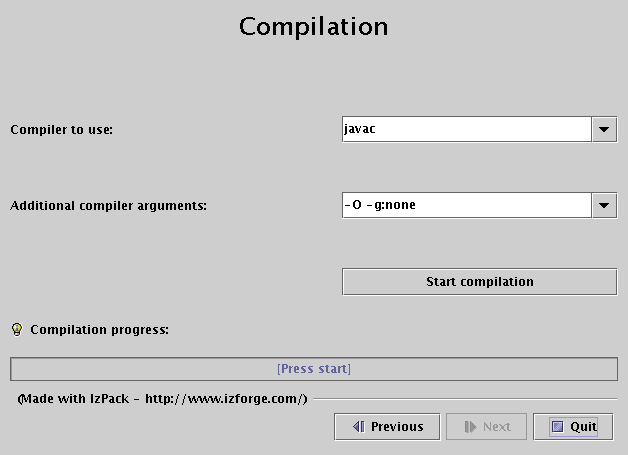
\includegraphics[width=\linewidth]{img/compilePanel}

\subsection{ProcessPanel}

This panel allows you to execute arbitrary files after installation.
The details for the compilation are specified using the resource \texttt{ProcessPanel.Spec.xml}.

The XML file has the following format:
\begin{verbatim}
<processing>
  <job name="do xyz">
    <os family="windows" />
    <executefile name="$INSTALL_PATH/scripts/xyz.bat">
      <arg>doit</arg><arg>$variable</arg>
    </executefile>
  </job>
  <job name="do xyz">
    <os family="unix" />
    <executefile name="$INSTALL_PATH/scripts/xyz.sh">
      <arg>doit</arg><arg>$variable</arg>
    </executefile>
  </job>
</processing>
\end{verbatim}

Each job may have an \texttt{<os>} attribute -- see \ref{tag:os} for details.\\

It is also possible to execute Java classes from this panel. Here's what this
feature author (Alex Bradley) says:
\begin{quotation}
I've been able to work around my requirements by extending the
\texttt{ProcessPanelWorker} functionality to run user-specified classes. I've
extended the DTD of the \texttt{ProcessPanel.Spec.xml} to include a new element:
\begin{verbatim}
<executableclass name="classname">
<args..../>
</executableclass>
\end{verbatim}
I've also added a new sub-class of \texttt{Processable} called
\texttt{ExecutableClass}. This will run a user-specified class in the context of
the installer JVM with a single method :
\begin{verbatim}run( AbstractUIHandler handler, String[] args]);\end{verbatim}

It can do everything I need and more. In particular, it allows me to write a
process extension and still be able to provide feedback to the user through
the feedback panel, and to add new functionality to the installer, after its
been built.
\end{quotation}

  % Chapter 3
\chapter{Advanced Features}

% Ant Integration
\section{Ant Integration}

\IzPack can be easily integrated inside an Ant build process. To do so you
first need to tell Ant that you would like to use \IzPack :
\footnotesize
\begin{verbatim}
<!-- Allows us to use the IzPack Ant task -->
<taskdef name="izpack" classpath="${basedir}/lib/compiler.jar"
         classname="com.izforge.izpack.ant.IzPackTask"/>
\end{verbatim}
\normalsize

Don't forget to add \texttt{compiler.jar} to the classpath of the Ant process.\\

Then you can invoke \IzPack with the \texttt{izpack} task which takes the
following parameters :
\begin{itemize}

  \item \texttt{input} : the XML installation file
  \item \texttt{output} : the output jar installer file
  \item \texttt{installerType} : the installer type
  \item \texttt{baseDir} : the base directory to resolve the relative paths
  \item \texttt{izPackDir} : the \IzPack home directory.
  
\end{itemize}\

Here is a sample of the task invocation :\\
\footnotesize
\begin{verbatim}
<!-- We call IzPack -->
<echo message="Makes the installer using IzPack"/>
<izpack input="${dist.dir}/IzPack-install.xml"
        output="${dist.dir}/IzPack-install.jar"
        installerType="standard-kunststoff"
        basedir="${dist.dir}"
        izPackDir="${dist.dir}/"/>
\end{verbatim}
\normalsize

% Automated Installers
\section{Automated Installers}

When you conclude your installation with a FinishPanel, the user can
save the data for an automatic installation. With this data, he will be
able to run the same installation on another similar machine. In an
environment where many computers need to be supported this can save
\textsl{a lot} of time.\\

So run once the installation on a machine and save your automatic installation
data in \texttt{auto-install.xml} (that's just a sample). Then put this file in
the same directory as the installer on another machine. Run it with :\\
\texttt{java -jar installer.jar auto-install.xml}\\

It has reproduced the same installation :-)\\

% Picture on the Language Selection Dialog
\section{Picture on the Language Selection Dialog}

You can add a picture on the language selection dialog by adding the following
resource : \texttt{installer.langsel.img}. \textsl{GIF}, \textsl{JPEG} and
\textsl{PNG} pictures are supported starting from J2SE 1.3.\\

% Installer picture
\section{Picture in the installer}

It is possible to specify an optional picture to display on the left side of the
installer. To do this, you just have to define a resource whose id is
\texttt{Installer.image}. For instance,
\begin{verbatim}
<res id="Installer.image" src="nice-image.png" />
\end{verbatim}
will do that. If the resource isn't specified, no picture will be displayed at
all. \textsl{GIF}, \textsl{JPEG} and
\textsl{PNG} pictures are supported starting from J2SE 1.3.\\

You can also give a specific picture for a specific panel by using the
\texttt{Installer.image.n} resource names where $n$ is the panel index. For
instance if you want a specific picture for the third panel, use
\texttt{Installer.image.2} since the indexes start from 0.\\

% Web Installers
\section{Web Installers}

The web installers allow your users to download a small installer that does not
contain the files to install. These files will be downloaded from a HTTP server
such as \textit{Apache HTTPD}. If you have many optional packs, this can save
people's resources. It's really easy : people download a small Jar
file containing the installer, they launch it and choose their
packages. Then the installer will get the files from another Jar file
located on a server. It's that simple.\\

Now suppose that you want to make an installer for your application
that you want to be named \texttt{install.jar}.
\begin{enumerate}
  \item open your favorite text editor and make a plain text file
  containing on the first line the URL to where you want to put the
  Jar file containing your packs, let's say for instance
  \url{http://www.mywebsite/myapp/install_web.jar}
  \item add this text file as a resource named
  \texttt{WebInstallers.url}
  \item compile your installer : you get \texttt{install.jar} and
  \texttt{install\_web.jar}
  \item copy \texttt{install\_web.jar} to
  \url{http://www.mywebsite/myapp/install_web.jar} and give your
  users \texttt{install.jar} for download.
\end{enumerate}\

That's all you need to make web installers.
Please note that the installation can look like frozen while the installer
grabs the server part.\\

% More Internationalization
\section{More Internationalization}

\subsection{Special resources}

IzPack is available in several languages. However you might want to
internationalize some additional parts of your installer. In particular you
might want this for the *InfoPanel and *LicencePanel. This is actually pretty
easy to do. You just have to add one resource per localization, suffixed with the
ISO3 language code. At runtime these panels will try to load a localized version.\\

For instance let's suppose that we use a HTMLInfoPanel. Suppose that we have it
in English, French and German. We want to have a French text for french users.
Here we add a resource pointing to the French text whose name is
\texttt{HTMLInfoPanel.info\_fra}. And that's it ! English and German users (or
anywhere other than in France) will get the default text (denoted by 
\texttt{HTMLInfoPanel.info}) and the French users will get the French version.
Same thing for the other Licence and Info panels.\\

\noindent
\textit{To sum up :} add \texttt{\_<iso3 code>} to the resource name for
\texttt{InfoPanel}, \texttt{HTMLInfoPanel}, \texttt{LicencePanel} and
\texttt{HTMLLicencePanel}.\\

\subsection{Packs}

Thanks to Thorsten Kamann, it is possible to translate the packs names and
descriptions. To do that, you have to define a special identifier in the
elements of the XML installation file and add the related entries in the
suitable langpacks. For instance if you have the following XML snippet:
\begin{verbatim}
<pack name="core" id="core.package" ...>
  <description/>
</pack>
\end{verbatim}
then the related entries of the langpacks will look like this:
\begin{verbatim}
<str id="core.package" txt="Core Package"/>
<str id="core.package.description" txt="The core package provides
\end{verbatim}

  % IzPack - Documentation

% Shortcut definition

\chapter{Desktop Shortcuts} (by Elmar \textsc{Grom})\\

\section{Defining Shortcuts}

\subsection{Introduction}

On todays GUI oriented operating systems, users are used to launching
applications, view web sites, look at documentation and perform a
variety of other tasks, by simply clicking on an icon on the desktop or
in a menu system located on the desktop. Depending on the operating
system these icons have different names. In this context I will refer to
them collectively as shortcuts.\\

Apart from actually placing an application on the target system, users
routinely expect an installer to create the necessary shortcuts for the
application as well. For you as application developer, this means that
for a professional appearance of your product you should also
consider creating shortcuts.\\

In contrast to the general specification of an IzPack installer, the
specification of shortcuts in IzPack requires a little more effort. In
addition, some of the concepts are a bit more complex and there are some
operating system specific issues to observe. Fortunately, you only need
to worry about operating system specifics if you want to deploy your
application to multiple different operating systems. In any case, it
will pay off to spend some time to study this documentation and the
example spec file before you start to implement your own shortcuts.\\

At the time of this writing (for IzPack version 3.0) IzPack is only
capable of creating shortcuts on the Microsoft Windows operating systems
[Win95 and higher and Win-NT 4.0 and higher]. Other operating systems,
such as Mac and UNIX flavors are not directly supported. However, there
is a special UI that automatically pops up on unsupported systems. It
informs the user about the intended targets of your shortcuts and allows
the user to save this information to a text file. While this is not an
elegant solution, at least it aids the user in the manual creation of
the shortcuts.\\

If you would like to review what an end user would see if the target
operating system is not supported, you can do the following. Simply
place the tag \texttt{<notSupported/>} in the spec file. This tag requires no
attributes or other data. It must be placed under \texttt{<shortcuts>}, just like
the individual shortcut specifications. Be sure to remove this tag
before getting your application ready for shipment.\\

We expect other operating systems to be supported in the near future and
as always, contributions are very welcome. At present someone is
actively working on Mac support and  Julien wanted to implement a
solution for KDE.\\

\subsection{What to Add to the Installer}

There are a number of things that you must add to the installer to make
it ready for creating shortcuts. Obviously you need to add the panel
responsible for creating shortcuts. This panel is aptly enough called
ShortcutPanel. However, in order for the ShortcutPanel to function
properly a number of additional items are required. These must be added
manually to the installer, because the front-end does not support this
feature yet. In this chapter I will explain which of these items are
required and for what reason.\\

First, I would like to discuss items that are supplied with IzPack and
only need to be added to the installer. After that, I move on to the
things you have to prepare yourself before you can add them. The way in
which shortcuts are created varies widely among operating systems. In
some cases it is actually possible to do this with pure Java code, while
other systems -such as MS-Windows- require native code to accomplish
this task. The native libraries required for the supported operating
systems are supplied with IzPack but they are not automatically added to
your installer file. You need to list them yourself in the XML file for
the installer. I'll describe later how to do this. At the time of this
writing (for IzPack version 3.0) only MS-Windows is supported. The
native library required for this operating system is called
\texttt{ShellLink.dll}.\\

Native libraries can be added to the installer by using the
\texttt{<native>} tag. To add the DLL for Windows for example, you just
have to add the following line to the installer XML file:\\
\texttt{<native type="izpack" name="ShellLink.dll"/>}\\
For more details about the use of the \texttt{<native>} tag see the
chapter about the format of the XML file.\\

You have to supply an extra specification file for the shortcuts that
you want to be  created on the target system. This file is required by
the shortcut panel. The format for this spec file is XML. It must be
added to the installer as a resource. The source name of this
specification does not matter, however its name when added to the
installer must be \texttt{shortcutSpec.xml}. This is the name the
ShortcutPanel looks for, do not use a different name and do not a path
to the name! If the specification file can not be found, the
ShortcutPanel will not show at all.\\

\textbf{Example}\\

\footnotesize
\begin{verbatim}
<res src="C:\MyDocuments\Installer\MyShortcutSpec.xml" 
     id="shortcutSpec.xml"/>
\end{verbatim}
\normalsize

\subsection{Why Native Code to do the Job?}

This little chapter is not strictly part of the documentation but I have
been asked this question sufficiently often that I think it's worth
explaining right here. It is certainly a natural question to ask. After
all IzPack is an application completely written in Java and primarily
targeted for the installation of Java based programs. So why wouldn't we
try to keep everything pure Java and avoid the use of native code
altogether? There must be some personal preference of the developer
hidden behind this approach you might think. Well, not really, but I
admit at first it seems quite feasible to write it all in Java. On
virtually any operating system or GUI surface around, Shortcuts are
simply files on the local file system. Files can be created and accessed
directly from within Java, so why should there be a need for using
native code?\\

Well, it turns out that just creating a file is not good enough, it also
needs to have the right content. Shell Links as they are called in
Windows land are binary files. I actually managed to find documentation
on the format. Naturally this was hacker data, you won't get this sort
of thing from Microsoft (by the way: thanks a lot to Jesse Hager for a
smash job!). Armed with this information I tried to create these files
myself in Java. The problem was that the documentation was not entirely
accurate and had some gaps as well. I tried for over a month to get this
to work but finally I had to give up. Even if I would have succeeded, it
would have been a hack, since a shell link requires some information that
is impossible to obtain from within Java. Usually you can successfully
create a shell link by only filling in the bare minimum information and
then ask Windows to resolve the link. Windows then repairs the shell
link. Unfortunately this was only the beginning, soon I encountered a
host of other problems. For one thing, the installer needs to know the
correct directories for placing the links and it turns out they are
named differently in different countries. In addition, there are ways of
manually modifying them, which some people might actually have done. The
only way to place the shortcut files reliably is through accessing the
Windows Registry. Naturally, this operation also required native code.
Same thing with asking Windows to resolve the link... On the bottom
line, at every step and turn you run into an issue where you just need
to use native code to do the trick. So I decided that I would do it the
proper way all the way through. That is in a nutshell the reason why I
used native code to create shortcuts on MS-Windows.\\

As I am writing this I am at work with a friend to replicate this work
for the Mac and it looks very much like we need to take the same
approach there as well. The various UNIX GUI surfaces on the other hand
seem promising. It might turn out that we can do the job without native
libraries, we will see...\\

\subsection{The Shortcut Specification}

The specification for shortcuts is provided to the ShortcutPanel in the
form of a XML file. At the time of this writing (for IzPack version 3.0)
the front-end has no support for generating this specification. Until a
later version provides front-end support you will have to write the
specification manually. For your convenience, an annotated sample
specification is located in the sample subdirectory of your IzPack
installation. At the beginning you might want to experiment with that
file.\\

The specification file has only one major section called \texttt{<shortcuts>}.
In this section, two different tags are recognized: \texttt{<programGroup>} and
\texttt{<shortcut>}.\\

The \texttt{<programGroup>} tag allows you to specify the name of the
menu under which the shortcuts will be grouped. The exact location and
appearance of the program group depends on the specific target system on
which the application will be installed, however you have some influence
on this. Please note that \texttt{<programGroup>} may only appear once
in the specification. If more than one instance occurs, only the first
one will be used. This tag requires two attributes: \texttt{defaultName}
and \texttt{location}. \texttt{defaultName} specifies the name that the
group menu should have on the target system. You should be aware that
the ShortcutPanel will present this name to the user as a choice. The
user can then edit this name or select a group that already exists. As a
result, there is no guarantee that the actual name of the program group
on the target system is identical with your specification.
\texttt{location} specifies where the group menu should show up. There
are two choices: \texttt{applications} and \texttt{startMenu}. If you
use \texttt{applications}, then the menu will be placed in the menu that
is ordinarily used for application shortcuts. If you use
\texttt{startMenu}, the group menu will be placed at the top most menu
level available on the target system. Depending on the target system, it
might not be possible to honor this specification exactly. In such
cases, the ShortcutPanel will map the choice to the location that most
closely resembles your choice.\\

For each shortcut you want to create, add one \texttt{<shortcut>} tag.
Most details about the shortcut are listed as attributes with this tag.
The following sections describe what each attribute does, which
attributes are optional and which ones are required and what the values
are that are accepted for each of the attributes. Note that all
attributes that have a yes/no choice can also be omitted. Doing so has
the same effect as using a value of no. The shortcut attributes can be
divided into two groups\\

\begin{itemize}
\item attributes that describe properties of the shortcut
\item attributes that define the location(s) at which a copy of the
      shortcut should be placed.
\end{itemize}\

The following attributes are used to define location:
\begin{itemize}
\item \texttt{programGroup}
\item \texttt{desktop}
\item \texttt{applications}
\item \texttt{startMenu}
\item \texttt{startup}
\end{itemize}\

\subsection{Shortcut Attributes}

There are three classes of attributes. Some are required, most are
completely optional and some are semi-optional. The set of semi-optional
attributes are all the attributes used to define the location of a
shortcut. These are semi-optional because for any individual one it is
your choice if you want to include it or not. However they are not
completely optional. You must specify at least one location. If all were
omitted, the instruction would essentially tell the panel that a copy of
this shortcut is to be placed at no location. In other words no copy is
to be placed anywhere.

\textbf{name} \texttt{- required}\\

The value of this attribute defines the name that the shortcut will
have. This is the text that makes up the menu name if the shortcut is
placed in a menu or the caption that is displayed with the shortcut if
it is placed on the desktop.\\

\textbf{target} \texttt{- required}\\

The value of this attribute points to the application that should be
launched when the shortcut is clicked. The value is translated through
the variable substitutor. Therefore variables such as
\texttt{\$INSTALL\_PATH} can be used to describe the location.
\textbf{You should be aware that the use of this tag is likely to change
once other operating systems are supported}.\\

\textbf{commandLine} \texttt{- optional}\\

The value of this attribute will be passed to the application as command
line. I recommend to work without command line arguments, since these are
not supported by all operating systems. As a result, your applications
will not be portable if they depend on command line arguments. Instead,
consider using system properties or configuration files.\\

\textbf{workingDirectory} \texttt{- optional}\\

This attribute defines the working directory for the application at the
time it is launched. I would recommend some caution in relying on this
too heavily if your application should be portable, since this might not
be supported by all operating systems. At this time I don't have enough
information to make a definite statement one way or the other. The value
is translated through the variable substitutor. Therefore variables such
as \texttt{\$INSTALL\_PATH} can be used to describe the directory.\\

\textbf{description} \texttt{- optional}\\

The value of this attribute will be visible to the user when a brief
description about associated application is requested. The form of the
request and the way in which this description is displayed varies
between operating systems. On MS-Windows the description is shown as a
tool tip when the mouse cursor hovers over the icon for a few seconds.
On some operating systems this feature might not be supported but I
think it is always a good idea to include a brief description.\\

\textbf{iconFile} \texttt{- optional}\\

The value of this attribute points to the file that holds the icon that
should be displayed as a symbol for this shortcut. This value is also
translated through the variable substitutor and consequently can contain
variables such as \$INSTALL\_PATH. If this attribute is omitted, no icon
will be specified for the shortcut. Usually this causes the OS to
display an OS supplied default icon. \textbf{The use of this attribute
is also likely to change once other operating systems are supported}.\\

\textbf{iconIndex} \texttt{- optional}\\

If the file type for the icon supports multiple icons in one file, then
this attribute may be used to specify the correct index for the icon. I
would also advise against using this feature, because of operating
system incompatibilities in this area. In file formats that do not
support multiple icons, this values is ignored.\\

\textbf{initialState} \texttt{- optional}\\

There are four values accepted for this attribute: \texttt{noShow},
\texttt{normal}, \texttt{maximized} and \texttt{minimized}. If th
target operating system supports this feature, then this value will have
the appropriate influence on the initial window state of the
application. \texttt{noShow} is particularly useful when launch scripts
are used that cause a command window to open, because the command window
will not be visible with this option. For instance on MS-Windows
starting a batch file that launches a Java application has the less than
pretty side effect that two windows show: the DOS command prompt and the
Java application window. Even if the shortcut is configured to show
minimized, there are buttons for both windows in the task bar. Using
\texttt{noShow} will completely eliminate this effect, only the Java
application window will be visible.\\

\textbf{programGroup} \texttt{- semi-optional}\\

The value for this attribute can be either yes or no. Any other value
will be interpreted as no. If the value is yes, then a copy of this
shortcut will be placed in the group menu.\\

\textbf{desktop} \texttt{- semi-optional}\\

For this attribute the value should also be yes or no. If the value is
yes, then a copy of the shortcut is placed on the desktop.\\

\textbf{applications} \texttt{- semi-optional}\\

This is also a yes/no attribute. If the value is yes, then a copy of the
shortcut is placed in the applications menu (if the target operating
system supports this). This is the same location as the applications
choice for the program group.\\

\textbf{startMenu} \texttt{- semi-optional}\\

This is a yes/no attribute as well. If the value is yes, then a copy of
the shortcut is placed directly in the top most menu that is available
for placing application shortcuts.\\

\textbf{startup} \texttt{- semi-optional}\\

This is also a yes/no attribute. If the value is yes, then a copy of the
shortcut is placed in a location where all applications get automatically
started at OS launch time, if this is available on the target OS.\\

\subsection{Selective Creation of Shortcuts}

Usually all shortcuts that are listed will be created when the user
clicks the 'Create Shortcuts' button. However it is possible to control
to some degree if specific shortcuts should be created or not. This is
based on install conditions. By including one or more \texttt{<createForPack>}
tags in the specification for a shortcut, you can direct the
ShortcutPanel to create the shortcut only if any of the listed packs are
actually installed. The 'name' attribute is used to define the name of
one of the packs for which the shortcut should be created. You do not
need to list all packs if a shortcut should always be created. In this
case simply omit this tag altogether.\\

\textbf{A word of caution}\\

For any shortcut that is always created, I would recommend to omit this
tag, since I have seen a number of problems related to changing pack
names. You can save yourself some troubleshooting and some Aspirin by
not using this feature if it's not required. On the other hand if you
need it I would advise to be very careful about changing pack names.\\

\subsection{Summary}

\textbf{Native Libraries}
\begin{itemize}
\item ShellLink.dll \texttt{- Microsoft Windows}
\end{itemize}\

\textbf{Name of Specification File}\\
\texttt{shortcutSpec.xml}\\

\textbf{Specification File Layout}
\footnotesize
\begin{verbatim}
<shortcuts>
  <programGroup defaultName="Name of the Program Group" 
                location="applications/startMenu"/>
  <shortcut 
    name="the name"
    target="the application to launch"
    commandLine=""
    workingDirectory="c:\MyWorkingDirectory\data"
    description="a description for the shortcut"
    iconFile="the file that contains an icon for the shortcut" 
    iconIndex="0"
    initialState="noShow/normal/maximized/minimized"
    programGroup="yes/no"
    desktop="yes/no" 
    applications="yes/no" 
    startMenu="yes/no" 
    startup="yes/no">
  
    <createForPack name="a pack name"/>
    <createForPack name="another pack name"/>
  </shortcut>
</shortcuts>
\end{verbatim}\
\normalsize

\section{Shortcut Tips}

I wrote this section to provide additional information about issues
surrounding the creation of shortcuts. Reading this section is not
necessary to successfully create shortcuts, but it might help you
creating an installation that works more smoothly. In addition, it might
give you some knowledge about operating systems that you don't know so
well. In fact most of the issues described in this section are focused
on differences in operating system specifics.\\

\subsection{The Desktop}

You should recognize that the desktop is precious real estate for many
people. They like to keep it uncluttered and keep only the things there
that they use on a regular basis. This is not true for everybody and you
might personally think different about this. Still, the fact remains
that a lot of people might have different feelings about it, so you
should not automatically assume that it is ok to place all of your
shortcuts on the desktop proper. While your application is certainly one
of the most important things for you, for your customers it is probably
one of many applications they use and maybe not even the most important
one. Accordingly, placing more shortcut icons there than they feel they
will use on a regular basis and especially doing this without asking for
permission might trigger some bad temper.\\

It is common practice to create a program group on the application menu
system of the OS and place all shortcuts that go with an application in
that program group. In addition, only one shortcut to the key access
point of the application is placed directly on the desktop. Many
installers first ask for permission to do so, as does the ShortcutPanel
in IzPack.\\

I would like to recommend that you always create a shortcut in the menu
system, even if your application has only one access point and you are
placing this on the desktop. Note that shortcuts can be placed directly
in the menu, they don't need to be in a program group. There are two
reasons for doing so.\\

\begin{itemize}
\item If the user elects not to create shortcuts on the desktop, they
      will end up with no access point to your application
\item Even if this works fine, occasionally people 'clean up' their
      desktop. They might later find that they accidentally deleted the
      only access point to your application. For the less technology
      savvy users, recreating the shortcut might be a rough experience.
\end{itemize}\

\subsection{Icons}

Icons are supplied in image files, usually in some kind of bitmap
format. Unfortunately there is no format that is universally recognized
by all operating systems. If you would like to create shortcuts on a
variety of operating systems that use your own icons, you must supply
each icon in a number of different formats. This chapter discusses icon
file formats used on various operating systems. Fortunately there are
good programs available that allow you to convert between these formats,
so that creating the different files is not much of a problem once the
icons themselves are created.\\

\textbf{Microsoft Windows}\\

Windows prefers to use its native icon file format. Files of this type
usually use the extension *.ico. Icon files can hold multiple icons in
one file, which can be useful if the same icon is to be provided in a
number of sizes. The iconIndex attribute in the spec file allows you to
specify which of the icons to use.\\

Windows also supports the use of bitmap files in the *.bmp format as
icons. Note that this format does not support multiple icons.\\

I am not a total expert in this area and might have overlooked other file
formats that are supported by Windows. However, I would suggest to test
other formats for compatibility as they might not work all the way back
to Windows 95 or on the NT/non-NT strain. Sticking with one of these two
formats should keep you out of trouble.\\

\textbf{Apple}\\

Apple Macintosh systems use the Macintosh PICT format, extension *.pct.
If you are working with an apple system you know a whole lot more about
this format than I do. If you don't but would like to be able to install
your application on a Mac, simply start with any bitmap format that you
feel comfortable to work with. Then find an application that is capable
of converting this format into a *.pct file. I like to use Paint Shop
Pro (PC based), because it provides conversion capabilities among
several dozen different file formats.\\

\textbf{UNIX flavors}\\

Sorry folks at this time I have no information available on icon file
formats for the various UNIX GUI frontends. If anyone can provide
additional information the would be most welcome.\\

\subsection{Targets}

So, you thought you could escape the ugly mess of operating system
dependencies at least with the way how your Java application is started?
Sorry but I have just another bad message. The one positive thing is
that here you have a way of escaping, even if doing so has a few less
pretty side effects. At first, I would like to discuss various launching
options you have available on different operating systems. At the end of
the chapter I write about a way to make launching your application OS
independent.\\

\textbf{Microsoft Windows}\\

On Microsoft Windows you have a variety of options for launching your
application. Probably the most simple case is directly starting the Java
VM from the command line and typing out all parameters, such as class
path, the class name etc. In principle, this can be placed right in a
shortcut and should work.\\

A little more elegant solution is to place this in a batch file and have
the shortcut point to this batch file. This will also make it more
likely that users can repair or recreate shortcuts. Recreating shortcuts
with sophisticated command lines is practically impossible.\\

Another method is less commonly used but just as possible. Implement a
native executable that launches the VM with your Java application. The
VM comes as DLL and is used by java.exe in just the same way.\\

Clearly, even though the first option is a bit ugly and has some
drawbacks, it is the most portable solution among the three.\\

\textbf{Apple}\\

I am currently researching the details for the Mac environment. Expect
an updated chapter with the next release.\\

\textbf{UNIX}\\

UNIX provides essentially the same options as Windows. You can simply
use the command line option, you can write a shell script and you can
write a native launcher. Naturally this stuff is in no way compatible
with the equivalent Windows implementations. The native option is even
more problematic in this environment, since the code can not even be
moved from one UNIX platform to another, without recompilation.\\

\textbf{OS Independent Launching}\\

So, after all this rather discouraging news, there is actually a
portable way to launch Java applications? You bet! although I have to
admit that it is not necessarily the most pretty way of doing things.\\

This approach is actually used by IzPack. Package your application in a
*.jar file if you don't already do so and make it executable. I am not
going into all the details on how exactly to do this, the Java
documentation will have to do. You might have noticed that even though
the instructions to install IzPack say to type :
\begin{verbatim}
java -jar IzPack-install.jar
\end{verbatim}\\

You can just as well double click on IzPack-install.jar and it will
start up. This procedure will work on all Java supported operating
systems -though you might have to replace double clicking with dropping
the file on the VM. In just the same way, you can make the *.jar file
itself the target of a shortcut.\\

The one drawback with this approach is that a *.jar file can only have
one main file. So, if you have multiple targets, they need to be
packaged each into a different *.jar file. They can be in one *.jar file
but then you have to start them explicitly, which gets you back to the
problems that I mentioned before. This brings me to the ugly part. If
you have just one target, then you are all set. If you have multiple
targets, you need to create a *.jar file for each of them. In addition,
you have a much harder time setting the classpath, because each of the
*.jar files that contain supporting code must be listed. In fact, at
present there is no way of setting this during the installation, because
IzPack does not yet (version 3.0) support the setting and modification
of environment variables.\\

\subsection{Command Line}

Before I start to write a lot about the use of command line arguments
let me state this: If you can avoid using them, do it! Not that there
is anything wrong with command line arguments as such. The issue is
simply that if you want your application to be usable cross platform
(the big Java promise) you should shy away from using command line
arguments. The problem here is that not all operating systems actually
support command line arguments. To be more precise, to my knowledge only
Apple operating systems do not support command line parameters. If you
don't care for running your application on a Mac, then you might not
worry about his at all. If you are interested to support the Mac as
well, read on.\\

In fact the Mac supports command line parameters in a way. More to the
point, it supports a single parameter that your application should
interpret as the name of a data file to open. You have no way of
supplying this to your application through the command line attribute.
The operating system generates this when the user drops the file on your
application and then passes it as command line argument. That's it. This
same behavior will probably fly well on pretty much any system and
should therefore be an ok implementation.\\

So what to do if you want to modify program behavior based on runtime
switches? For one thing, you could set system properties accordingly.
The drawback here is the same as with the command line parameters: the
way of setting these might vary between operating systems. The best way
seems to be using a property file that contains the configuration
data.\\

\section{Trouble Shooting}

It has been some time since I wrote this chapter during which a good
number of users had a chance to gather experience. Unfortunately I
never know how many have used it successfully without much difficulty. I
only hear from those that have encountered one problem or another. The
type of problems that I have seen prompted me to write this section,
because I think it will help you in locating most problems that you might
encounter or at least give you some idea where the problem might be
located.\\

\subsection{Problems You Can Solve}

If you see an exception that essentially says that a library can not be
loaded (ShellLink.dll) you have an easy problem to deal with. Your
installer file is probably missing the native tag that adds the Windows
dll to the installer or something with this tag is no quite right. Read
'What to Add to the Installer' for all details on this topic.\\

Most other problems cause the ShortcutPanel not to show at all during
the installation process. The reason is simply that the ShortcutPanel
skips if it does not know what to do or if it has nothing to do (no
point showing then and confusing the user). The problem is that this is
not always what you intended. In the most simple but not so uncommon
case the ShortcutPanel cannot find the spec file. This can be caused by
a number of reasons. The associated resource tag might be missing in the
installer specification, the target file name might be misspelled (the
name you specify for the \texttt{id} attribute) or the target file name
has a path or package name pre-pended. Just use
\texttt{shortcutSpec.xml} and nothing else, just as described in 'What
to Add to the Installer'. You can always verify if this part is ok by
inspecting the content of the installer *.jar file. The file
shortcutSpec.xml should be located in the directory \texttt{res}. This
inspection can be performed with any zip tool. If the file is not there,
first correct this before proceeding.\\

If the file is there and the panel does not show you have a problem
within the specification file. In most cases that I have seen, it comes
down to a spelling mistake of an attribute or tag name. You just have to
carefully make sure that everything is spelled correctly. Don't forget
that all names are case sensitive! In a few cases it has also turned out
that required or semi-optional attributes are omitted, so you might want
to verify if all attributes that you need are actually supplied.\\

If everything is correct up to this point the problem becomes more
elusive.  Most likely the panel does not show because it is instructed
not to show. There are be several possible reasons for this. The simple
case is that no location has been specified for the shortcuts in your
installation. This can happen if all five location attributes are
omitted or if all the ones that are listed are set to \texttt{no}.
Remember, you must specify at least one location for every shortcut. If
this is also correct, you might have used the <creatForPack> tag. Review
the details in 'Selective Creation of Shortcuts'. One possibility for
the panel not to show is that based on the packs that are actually
selected for installation no shortcut qualifies for creation. In this
case the panel will not show, this is perfectly normal behavior. More
likely this condition is true because of some accident and not because
it's intended. Make sure the packs that you list for the shortcut are
actually defined in your installation and verify that they are all
spelled correctly. Remember: case matters! Did the ShortcutPanel use to
work in your installation and all of a sudden stopped working? Very
likely you are dealing with the last problem. A package name might have
been modified and the shortcut spec was not adjusted to stay in sync.\\

\subsection{Problems That Have No Solution (yet)}

Unfortunately one problem has been very persistent and only recently one
user found the reason. The problem occurs when installing on some target
systems where non-English characters are used in the storage path for
the shortcuts. The problem is that these characters don't seem to be
properly translated across the Java Native Interface. This leads to a
situation where the proper path can not be located and the shortcut
creation fails. I write 'some target systems' because it does not fail
everywhere. After much agonizing over this problem, one user found the
solution: The shortcut creation works fine if a Sun virtual machine is
installed, but fails if a version from IBM happens to be installed. So
far I have no solution for this problem but I am trying to find a
workaround the problem.\\

  % Chapter 5
\chapter{Making your own panels}

\section{How you can do that}

\subsection{Required stuffs}

You'll first have to read the NanoXML documentation if you need to use XML in
your panel. Secondly, it is necessary that you use the Javadoc-generated class
references. We will just explain here briefly how to start making your panels.\\

A good thing to do is to read the source code of some IzPack panels. They are
usually \textsl{very} small, so you'll understand easily how to do your owns.\\

\subsection{What you'll have to do}

Extending \IzPack with a panel is something really easy. Actually a panel is a
subclass of \texttt{IzPanel}. So all you have to do is make a subclass too. The
\texttt{IzPanel} class is located in the \texttt{com.izforge.izpack.installer}
package but your panels will have to belong to
\texttt{com.izforge.izpack.panels}.\\

A good thing to make the things easier for you is to work with the IzPack
building Jakarta Ant building process. Just add your class in the source tree
and add the And directives to build your own panels. This way you'll be able to
concentrate on code and nothing else :-)\\

\section{The \texttt{IzPanel} class}

\subsection{UML diagram}

\begin{center}
\fbox{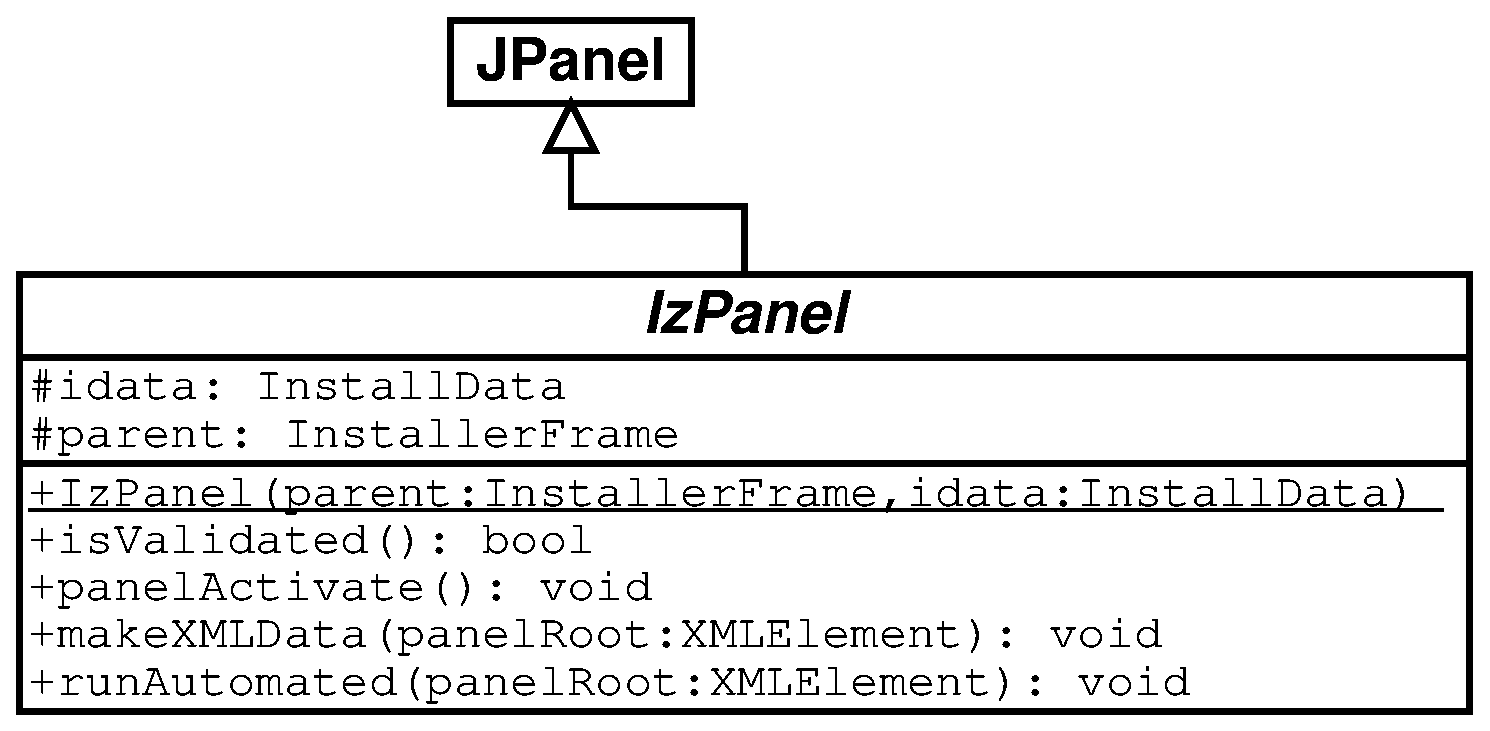
\includegraphics[scale=0.5]{img/ch5-izpanel.eps}}
\end{center}\

\subsection{Description}

The 2 members are : the installer data (refer to the \texttt{InstallData}
Javadoc reference) and the parent installer frame.\\

The methods have the following functions :\\
\begin{itemize}

  \item \textit{(constructor)} : called just after the language selection
  dialog. All the panels are built there and then the installer is shown. So
  take care of the fact that the installer window is \textbf{not} yet visible
  when the panel is created. If you need to do some work when the window exists,
  do it in \texttt{panelActivate}.\\

  \item \texttt{isValidated} returns \texttt{true} if the user is allowed to
  go a step further in the installation process. Returning \texttt{false} will
  lock it. For instance the LicencePanel returns \texttt{true} only if the user
  has agreed with the license agreement. Default is to return \texttt{true}.\\
  
  \item \texttt{panelActivate} is called when the panel becomes active. So
  implement here anything that suits here. Default is to do nothing.\\
  
  \item \texttt{makeXMLData} is called to build the automated installer data.
  Default is to do nothing. \texttt{panelRoot} refers to the node in the XML
  tree where you can save your data. Each panel is given a node. You can
  organize it as you want with the markups you want starting from
  \texttt{panelRoot}. It's that simple.\\
  
  \item \texttt{runAutomated} is called by an automated-mode installation. Each
  panel is called and can do its job by picking the data of the previous
  installation as saved in \texttt{panelRoot} by \texttt{makeXMLData}.\\

\end{itemize}\

  % IzPack - Documentation

% User Input

\chapter{\label{chap:userinput}User Input} (by Elmar \textsc{Grom})\\

Most of the panels that come with IzPack take user input in some form.
In some panels this is through a simple user acknowledgment in others
the user can enter text or select a directory through a file open
dialog. In all of those cases the user input is used for the specific
purpose  needed by the panel that takes the input. However, if you need
user input during installation that will later on be available  to your
application then you need to use the user input panel.\\

To use this panel, list it in the install file with the class name
\texttt{UserInputPanel}. In addition, you must write a XML specification
and add it to the install resources. The name of this resource must be
\texttt{userInputSpec.xml}.\\

The user input panel is a blank panel that can be populated with UI
elements through a XML specification file. The specification supports
text labels, input elements, explanatory text and some minor formatting
options.\\

The following types of user input elements are supported:
\begin{itemize}
\item Text
\item Combo Box
\item Radio Buttons
\item Check Box
\item Rule Input Field
\item Search Field
\end{itemize}\

The way in which this panel conveys the user input to your application
is through the variable substitution system. User input is not directly
inserted into your configuration files but the variables that you
specify for this panel are set in the variable substitution system.
After this operation has taken place the variables and associated values
are available for all substitutions made. This way of operation has a
number of implications that you should be aware of.\\

First, not only can you set additional variables in this way but you can
also modify variables that are defined elsewhere -even built in
variables. For this reason you should be careful to avoid overlaps when
choosing variable names. Although there might be cases when it seems
useful to modify the value of other variables, it is generally not a
good idea to do so. Because you might not exactly know when other
variables are set and when and where they are used throughout the
installation process, there might be unintended side effects.\\

Second, the panel must be shown at a point during the installation
process before the variables are used. In most cases you will use the
values to substitute variables in launch and configuration files that
you supply with your installation. For this to work you place this panel
before the install panel, because the install panel uses the variable
substitutor to replace all such variables. Although using this panel any
later in the process will correctly set the variables internally, there
won't be any affect on the files written to disk. You can also use
variables set in this way in other panels that you have written
yourself. There is a section in the  chapter on writing your own panel
that explains how to do this. Also in this case it is important to place
the associated input panel in the process before the variables are
used.\\

At this point I would also like to mention that it is possible to hide
select elements on the panel or the panel altogether if certain packs
are not selected. For this to work you must place this panel after the
packs panel. One side effect of using this feature is that it is not
possible to step back once the user input panel is displayed. This is
because the user might make changes in the packs selection that would
require a complete rebuild of the UI. Unfortunately, building the UI is
an irreversible process, therefore the user can not be allowed to go
back to the packs panel.\\


\section{The Basic XML Structure}

The top level XML section is called \texttt{<userInput>}. For most
panels it does not make sense to present them more than once, however
you might want to present multiple user input panels -with different
content of course. Therefore the \texttt{<userInput>} section can
contain multiple tags that each specify the details for one panel
instance. The tag name for this is \texttt{<panel>}.\\

The \texttt{<panel>} tag uses the following attributes:\\

\textbf{order} \texttt{- required}\\

This is the order number of the user input panel for which this
specification should be used. Counting starts at 0 and increments by 1
for each instance of the user input panel. So if a spec should be used
for the second occurrence of the user input panel use
\texttt{order="1"}.\\

\textbf{layout} \texttt{- optional}\\

There are three general layout rules this panel uses, they are
\texttt{left}, \texttt{center} and \texttt{right}. While I think left is
most commonly used, you might want to experiment with this attribute and
see which you like best. The default is \texttt{left}.\\


\section{Concepts and XML Elements Common to All Fields}

Before I dive into the details of defining the various UI elements I
would like to present XML elements and general concepts that apply
throughout. This saves me a lot of work in writing and you a lot of
repetitive reading and maybe a tree or two.\\

The UI elements are generally laid out top to bottom in the order they
appear in the XML file. The only exception to this rule is the title,
which always appears at the very top. The layout pattern for the input
fields is as follows: If a description is defined, it appears first,
using the full available layout width. The input field is placed beneath
the description. With fields such as the text field or the combo box,
the label is placed to the left and the input field to the right. Fields
such as radio buttons and check boxes are somewhat indented and have the
label text appear to their right.\\

Each UI element is specified with a \texttt{<field>} tag. The
\texttt{type} attribute is used to specify what kind of field you want
to place. Obviously, the \texttt{type} attribute is not optional.\\

Each field that takes user input must also specify the variable that
should be substituted. This is done with the \texttt{variable}
attribute.\\

\label{userInput:descriptiontag}
Almost all fields allow a description. When a description is allowed it
is always added in the same way. The description is part of the data
within the field tag. There can only be one description per field. If
you add more than one, the first one is used and the others ignored.
There are three attributes used with this tag. The text is specified
through the \texttt{txt} or the \texttt{id} attribute. The details on
using them are described below. The attributes are all optional but you
must specify text to use, either directly or through the \texttt{id}
attribute. In addition, you can set the text justification to
\texttt{left}, \texttt{center} and \texttt{right} with the
\texttt{align} attribute. \\

The following example illustrates the general pattern for field specification:\\

\footnotesize
\begin{verbatim}
<field type="text" variable="myFirstVariable">
  <description align="left" txt="A description" id="description 1"/>
  .
  .
  .
</field>
\end{verbatim}
\normalsize

A very frequently used pattern is for the definition of text. Where ever
text is needed (labels, descriptions, static text, choices etc.) it can
be specified in place using the \texttt{txt} attribute. This is
convenient if you are only supporting a single language. However, if you
would like to separate your text definitions from the panel
specification or if you need to support multiple languages you might
want to use the \texttt{id} attribute instead to only specify an
identifier. You can then add multiple XML files with the same name as
this spec file (userInputSpec.xml) appended with an unserscore '\_' and
the the appropriate three letter ISO3 language code. The content of
those files must conform to the specification for IzPack language
packages. For more details on this topic see the chapter on language
packages under advanced features. \texttt{id} defines an identifier that
is also defined in the language package, together with the localized
text to use. It is possible to use both the \texttt{txt} and the
\texttt{id} attribute. In this case the text from the language package
is used. If for some reason the language package is not available or the
\texttt{id} is not defined there, the text specified with \texttt{txt}
is used as default.\\

All input fields can be pre-set with a value of your choice. Although
the details vary a bit from field type to field type, the \texttt{set}
attribute is always used to accomplish this. The \texttt{set} attribute
is of course optional.\\

All fields that take user input use a \texttt{<spec>} tag to define the
details of the input field. In the some cases the content of this tag is
rather simple. Input fields with a more complex nature tend to have
accordingly complex content in this tag. Since the details vary widely,
they are explained with each input field.\\

Any number of \texttt{<createForPack>} tags can be added to the
\texttt{<panel>} and \texttt{<field>} sections. This tag has only one
attribute and no data. The attribute is \texttt{name} and specifies the
name of one of the installation packs that you have defined. Here is how
it works: if no \texttt{<createForPack>} tag exists in a section, the
entity is always created. However, if the tag exists, the entity is only
created if one or more of the listed packs are selected for
installation. As mentioned before, if you are using this feature, make
sure the user input panel shows up after the packs panel.\\

\section{Panel Title}

You can place an optional title at the top of the panel. Though it is
not possible to select a font for the title that is different form the
one used on the rest of the panel, it is possible to modify the font to
some extent. To specify the title create a \texttt{<field>} tag and use
the \texttt{type} attribute with the value \texttt{title}. In addition
to the \texttt{txt} and \texttt{id} attributes, the following attributes
are supported:\\

\textbf{italic} \texttt{- optional}\\

With a value of \texttt{true} specifies that the title font should be in italics.\\

\textbf{bold} \texttt{- optional}\\

With a value of \texttt{true} specifies that the title font should be bold.\\

\textbf{size} \texttt{- optional}\\

This attribute specifies the size of the title font. Please note that
the size is not specified in points but as a relative size multiplier
compared to the body font on the panel. The default value is 2.\\

\section{Static Text}

Static text is simply text that is placed on the panel without direct
connection to any of the input elements. It is laid out to use the
entire layout width available on the panel and is broken into multiple
lines if necessary. To specify static text create a \texttt{<field>} tag
and use the \texttt{type} attribute with a value of \texttt{staticText}.
In addition to the \texttt{txt} and \texttt{id} attributes, the text can
be justified \texttt{left}, \texttt{center} or \texttt{right} with the
\texttt{align} attribute. It is not possible to format this text in any way.\\

\textbf{Example}\\

The following example inserts some static text in the panel.

\footnotesize
\begin{verbatim}
<field type="staticText" align="left" 
       txt="This is just some simple static text."
       id="staticText.text"/>
\end{verbatim}
\normalsize

\section{Visual Separation}

Sometimes it is desirable to separate different entities visually. This
can be accomplished by inserting a space or a divider. A space simply
inserts a vertical separation of the average height of a single line
entity, such as a line of text or a an input field. A divider inserts
the same amount of space but also draws a division line which can be
either aligned at the top or bottom of the separation.
\texttt{<space>}, \texttt{<divider>}

 ..... maybe I should draw the line myself and add no additional space at all ...

\section{Text Input}

A text input field allows the user to enter and edit a single line of
text, without length restriction. The input field can have a label,
which will show to the left of the input field and a description, which
can span multiple lines. The description is placed above the input field
and uses the entire available layout width. The width of the input field
must be explicitly set, otherwise it will only accommodate a single
character. To specify a text input field create a \texttt{<field>} tag
and use the \texttt{type} attribute with a value of \texttt{text}. The
\texttt{txt} and \texttt{id} attributes are not supported here. The
\texttt{variable} attribute specifies the variable that should be
replaced with the text taken from the input field.\\

\textbf{The Data}\\

The data consists of two items, a description and the spec. The
\texttt{<spec>} tag uses four attributes. The label text is specified with
\texttt{txt} and/or \texttt{id} as described above. In addition, the
width of the input field as it appears on the panel can be set with the
\texttt{size} attribute. The value must be an integer and sets the field
width based on the average character width of the active font. If this
is not specified, then you will end up with a very narrow field that is
practically unusable.\\

The fourth attribute \texttt{set} is optional. It takes a text string to
pre-fill the input field.\\

\textbf{Example}\\

The following example creates a text input field with a label and
description. The width of the input field will be enough to accommodate
15 characters. The field will be pre-set with the text 'some text' when
the UI is first presented.\\

\footnotesize
\begin{verbatim}
<field type="text" variable="textInput">
  <description align="left" txt="A description for a text input field"
               id="description.text"/>
  <spec txt="Enter some text:" id="text.label" size="15" set="some text"/>
</field>
\end{verbatim}
\normalsize

\section{Radio Buttons}

The radio buttons are useful when the user needs to select a specific
option out of a pre-defined list of choices. This field offers an
arbitrary number of mutually exclusive buttons, each with its own label.
The placement of the buttons and labels is different form other fields.
First, the button is placed to the left and the label text to the right.
Second, the buttons are not lined up all the way to the left as other
labels are but they are indented from that location. As with other
fields, the description is placed above the list of radio buttons and
uses the entire available layout width. To specify a set of radio
buttons create a \texttt{<field>} tag and use the \texttt{type}
attribute with a value of \texttt{radio}. The \texttt{txt} and
\texttt{id} attributes are \textbf{not} supported here. As with all
other input fields, the \texttt{variable} attribute specifies that
variable that should be replaced with the user selection.\\

\textbf{The Data}\\

The data consists of two items, a description and the spec. The
\texttt{<spec>} tag has no attributes, instead the specification details
are entered as data within the \texttt{<spec>} tag. The \texttt{<spec>}
data consists of one or more \texttt{<choice>} tags. One
\texttt{<choice>} tag is required for each radio button. The
\texttt{<choice>} tag accepts the usual \texttt{txt} and \texttt{id}
attributes, which are used to specify the label text. In addition the
following attributes are supported:\\

\textbf{value} \texttt{- required}\\

The \texttt{value} attribute is used to specify which value to insert if
this associated radio button is selected. In other words, the label text
has nothing to do with the value that is actually substituted for the
variable. For this reason there is never an issue if multiple languages
are used, the value is always the same for a given selection.\\

\textbf{set} \texttt{- optional}\\

The \texttt{set} attribute accepts the values \texttt{true} and
\texttt{false}. Since the attribute is optional it can also be omitted,
which is interpreted as \texttt{false}. If a value of \texttt{true} is
used, the associated radio button will be selected when the UI is first
presented. Obviously, only one of the buttons in a set should be set to
\texttt{true}.\\

\textbf{Example}\\

The following example creates a set of four radio buttons with
description. The second button will be selected when the UI is first
presented.\\

\footnotesize
\begin{verbatim}
<field type="radio" variable="radioSelection">
  <description align="left" txt="This is a description for radio buttons"
               id="description.radio"/>
  <spec>
  <choice txt="the first choice" id="radio.label.1" value="1 selected" />
  <choice txt="the second choice" id="radio.label.2" value="2 selected"
          set="true" />
  <choice txt="the third choice" id="radio.label.3" value="3 selected" />
  <choice txt="the fourth choice" id="radio.label.4" value="4 selected" />
  </spec>
</field>
\end{verbatim}
\normalsize

\section{Combo Box}

The combo box provides essentially the same functionality as do the
radio buttons, just in a different presentation stile. The advantage of
the combo box is that it is easier to deal with a long list of
choices.\\

\section{Check Box}

If there are a number of choices and any combination of them could be
selected, not just a single one, then radio buttons are not the way to
go. You might be better off using a number of check boxes. The layout
for a check box works in the same way as for radio buttons. The check
box is placed indented from the left most edge and the label text is
placed to the right of it. Other than with radio buttons, you cannot
define any number of check boxes. This field allows the definition of
only one check box, which is associated with one variable. If you need
multiple check boxes you need to define one field for each of them.  To
make it look like a cohesive group you simply provide a description only
for the first check box. All of the check boxes will be positioned in
such a way that they look like a group, even though they are separate
entities and their selections are conveyed to different variables. The
description  is placed above the check box and uses the entire available
layout width. To specify a check box create a \texttt{<field>} tag and
use the \texttt{type} attribute with a value of \texttt{check}. As with
all other input fields, the \texttt{variable} attribute specifies the
variable that should be replaced with the user input.\\

\textbf{The Data}\\

The data consists of two items, a description and the spec. The
\texttt{<spec>} tag accepts the usual \texttt{txt} and \texttt{id}
attributes, which are used to specify the label text. In addition, the
following attributes are supported:\\

\textbf{true} \texttt{- required}\\

The \texttt{true} attribute specifies the value to use for substitution
when the box is selected.\\

\textbf{false} \texttt{- required}\\

The \texttt{false} attribute specifies the value to use for substitution
when the box is not selected.\\

\textbf{set} \texttt{- optional}\\

The \texttt{set} attribute accepts the values \texttt{true} and
\texttt{false}. Since the attribute is optional it can also be omitted,
which is interpreted as \texttt{false}. If a value of \texttt{true} is
used, the check box will be selected when the UI is first presented.\\

\textbf{Example}\\

The following example creates a check box with description. The check
box will not be selected when the UI is first presented. This could also
be accomplished by omitting the \texttt{set} attribute.\\

\footnotesize
\begin{verbatim}
<field type="check" variable="chekSelection.1">
  <description align="left" txt="This is a description for a check box"
               id="description.check.1"/>
  <spec txt="check box 1" id="check.label.1" true="on" false="off" 
        set="false"/>
</field>
\end{verbatim}
\normalsize

\section{Rule Input}

The rule input field is the most powerful and complex one of all the
input fields offered by this panel. In its most simple incarnation it
looks and works like a regular text input field. There is also only an
incremental increase of the complexity in the specification for this
case. However, it is unlikely that you would use it for such a purpose.
The real power of this input field comes from the fact that rules can be
applied to it that control many aspects of its look as well as overt and
covert operation.\\

\subsection{Layout and Input Rules}

The basic nature of this input field is that of a text input field and
as mentioned before, in its most simple incarnation that is what it
looks like and how it operates. However, the layout of the field can be
defined in such a way that there are multiple logically interconnected
text input fields, adorned with multiple labels. Further more, each of
these fields can be instructed to restrict the type of input that will
be accepted. Now you might ask what this could be useful for. As an
answer, let me present a few examples that show how this feature can be
used. Before I do this however, I would like to describe the
specification syntax, so that the examples can be presented together
with the specifications that make them work in a meaningful way.\\

The actual specification of the layout, the labels and the type of input
each field accepts all happens in a single string with the
\texttt{layout} attribute. First let us have a look at the specification
format for a single field. This format consists of a triplet of
information, separated by two colons ':'. A typical field spec would
look like this: \texttt{N:4:4}, where the first item is a key that
specifies the type of input this particular field will accept - numeric
input in the example. The second item is an integer number that
specifies the physical width of the field, this is the same as in the
with of any regular text field. Therefore the field in the example will
provide space to display four characters. The third item specifies the
editing length of the string or in other words, the maximum length of
the string that will be accepted by the field. In the \texttt{layout}
string you can list as may fields as you need, each with its own set of
limitations. In addition you can add text at the front, the end and in
between the fields. The various entities must be separated by white
space. The behavior of this field is such that when the editing length
of a field has been reached, the cursor automatically moves on to the
next field. Also, when the backspace key is used to delete characters
and the beginning of a field has been reached, the cursor automatically
moves on to the previous field. So let us have a look a some examples.\\

\textbf{Phone Number}

The following specification will produce a pre formatted input field to
accept a US phone number with in-house extension. Even though the
pattern is formatted into number groups as customary, complete with
parentheses '(' and dash '-', entering the number is as simple as typing
all the digits. There is no need to advance using the tab key or to enter
formatting characters. Because the fields only allow numeric entry, there
is a much reduced chance for entering erroneous information.
\texttt{"( N:3:3 ) N:3:3 - N:4:4 x N:5:5"}. Each of the fields uses the
'N' key, indicating that only numerals will be accepted. Also, each of
the fields only accepts strings of the same length as the physical width
of the field.\\

\begin{center}
\fbox{
\includegraphics[scale=1.0]{img/userInput-phone}}
\end{center}

\textbf{E-Mail Address}

This specification creates a pattern that is useful for entering an
e-mail address \texttt{"AN:15:U @ AN:10:40 . A:4:4"}. Even though the
first field is only fifteen characters wide it will accept a string of
unlimited length, because the 'U' identifier is used for the edit
length. The second field is a bit more restrictive by only accepting a
string up to forty characters long.\\

\begin{center}
\fbox{
\includegraphics[scale=1.0]{img/userInput-email}}
\end{center}

\textbf{IP Address}

It might not be uncommon to require entering of an IP address. The
following simple specification will produce the necessary input field.
All fields are the same, allowing just three digits of numerical entry.
\texttt{"N:3:3 . N:3:3 . N:3:3 . N:3:3"}\\

\begin{center}
\fbox{
\includegraphics[scale=1.0]{img/userInput-IP}}
\end{center}

\textbf{Serial Number or Key Code}

If you ship your product with a CD key code or serial number and require
this information for registration, you might want to ask the customer to
transcribe that number from the CD label, so that it is later on
accessible to your application. As this is always an error prone
operation, the predefined pattern with the easy editing support and
restriction of accepted data helps to reduce transcription errors
\texttt{"H:4:4 - N:6:6 - N:3:3"}. This particular specification will
produce three fields, the first accepting four hexadecimal, the second
six numerical and the third three numerical digits.\\

\begin{center}
\fbox{
\includegraphics[scale=1.0]{img/userInput-serial}}
\end{center}

\textbf{Limitations}

Even though the above examples all use single character labels between
fields, there is no restriction on the length of these labels. In
addition, it is possible to place label text in front of the first field
and after the last field and the text can even contain spaces. The only
limitation in this regard is the fact that all white space in the text
will be reduced to a single space on the display. This means that it is
not possible to use multiple spaces or tabs in the text.\\

The following table lists and describes all the keys that can be used in
the specification string.\\

\begin{center}
\begin{tabularx}{\textwidth}{|l|l|X|}
\hline \textit{Key} & \textit{Meaning} & \textit{Description} \\
\hline N & numeric & The field will accept only numerals.\\
\hline H & hexadecimal & The field will accept only hexadecimal numerals, that is all numbers from 0-F.\\
\hline A & alphabetic & The field will accept only alphabetic characters. Numerals and punctuation marks will not be accepted.\\
\hline AN & alpha-numeric & The field will accept alphabetic characters and numerals but no punctuation marks.\\
\hline O & open & The filed will accept any input, without restriction.\\
\hline U & unlimited & This key is only legal for specifying the editing length of a fields. If used, the field imposes no length restriction on the text entered.\\
\hline
\end{tabularx}\
\end{center}

\subsection{Setting Field Content}

Like all other input fields the rule input field can also be pre-filled
with data and as usual, this is accomplished thought the \texttt{set}
attribute. As you might expect, the details of setting this field are
rather on the complicated side. In fact you can set each sub field
individually and you can leave some of the fields blank in the process.
The \texttt{set} specification for all sub fields is given in a single
string. Each field is addressed by its index number, with the count
starting at 0. The index is followed by a colon ':' and then by the
content of the field. The string "0:1234 1:af415 3:awer" would fill the
first subfield with \texttt{1234}, the second one with \texttt{af415} and
the fourth with \texttt{awer}. The third subfield would stay blank
and so would any additional fields that might follow.\\

The individual field specs must be separated with spaces. Spaces within
the pre-fill values are not allowed, otherwise the result is undefined.\\

\subsection{The Output Format}

The user input from all subfields is combined into one single value and
used to replace the variable associated with the field. You can make a
number of choices when it comes to the way how the subfield content is
combined. This is done with the \texttt{resultFormat} and
\texttt{separator} attributes. The \texttt{resultFormat} attribute can
take the following values:\\

\begin{center}
\begin{tabularx}{\textwidth}{|l|X|}
\hline \textit{Value} & \textit{Meaning}\\
\hline \texttt{plainString} & The content of all subfields is simply concatenated into one long string.\\
\hline \texttt{displayFormat} & The content of all subfields and all labels -as displayed- is concatenated into one long string.\\
\hline \texttt{specialSeparator} & The content of all subfields is concatenated into one string, using the string specified withe the \texttt{separator} attribute to separate the content of the subfields.\\
\hline \texttt{processed} & The content is processed by Java code that you supply before replacing the variable. How to do this is described below.\\
\hline
\end{tabularx}\
\end{center}

\subsection{Validating the Field Content}

This feature needs to be documented.

\subsection{Processing the Field Content}

This feature needs to be documented.

\subsection{Summary Example}

\footnotesize
\begin{verbatim}
<field type="rule" variable="test1">
  <description align="left" txt="A description for a rule input field."
               id="description.rule.1"/>
  <spec txt="Please enter your phone number:" 
        layout="( N:3:3 ) N:3:3 - N:4:4 x N:5:5" 
        resultFormat="specialSeparator" separator="."/>
  <validator class="com.izforge.izpack.util.NotEmptyValidator"
             txt="The phone number is mandatory!" />
  <!--processor class=""/-->
</field>
\end{verbatim}
\normalsize

\section{Search}

The search input field allows the user to choose the location of files or
directories. It also supports auto-detection of the location using a list of 
suggestions. The field is basically a combobox with an extra button to
trigger auto-detection (again).

\begin{center}
\fbox{
\includegraphics[scale=0.8]{img/userInput-search}}
\end{center}

\subsection{Specification}

The \texttt{<description>} tag is the same as with other fields (see
\ref{userInput:descriptiontag} on page \pageref{userInput:descriptiontag}). The
\texttt{<spec>} tag supports the following attributes:

\begin{itemize}
\item \texttt{filename} - the name of the file or directory to search for
\item \texttt{type} - what to search for
  \begin{itemize}
  \item \texttt{file} - search for a file
  \item \texttt{directory} - search for a directory
  \end{itemize}
\item \texttt{result} - what to return as the search result
  \begin{itemize}
  \item \texttt{file} - result of search is whole pathname of file or directory found
  \item \texttt{directory} - only return directory where the file was found (this is the same as \texttt{file} when searching for directories)
  \item \texttt{parentdir} - return the full path of the parent directory where the file was found
  \end{itemize}
\item \texttt{checkfilename} - the name of a file or directory to check for existence (this can be used to validate the user's selection)
\end{itemize}

\subsection{Example}

\footnotesize
\begin{verbatim}
<field type="search" variable="java_sdk_home">
  <description align="left" 
               txt="This is a description for a search input field."
               id="description.java_sdk_home"/>
  <spec txt="Path to Java SDK:" checkfilename="lib/tools.jar"
        type="file" result="directory">
  <choice value="/usr/lib/java/" os="unix" />
  <choice value="/opt/java" os="unix" />
  <choice value="C:\Program Files\Java" os="windows" />
  <choice value="C:\Java" os="windows" />
  </spec>
</field>
\end{verbatim}
\normalsize


  % Appendixes
  \appendix
  \chapter{The GNU General Public License}
  \footnotesize
  \verbatiminput{GPL}
  \normalsize

\end{document}
